\chapter{Cosmological Background}

\section{Cosmological Principle}
The Cosmological principle states that the universe is homogeneous and isotropic on sufficiently large scales, larger than about \SI{100}{\mega\parsec}. This is a generalization of the Copernican principle, according to which there is no special place and no special direction in the universe.

In the following, the evolution of the universe will be described, assuming that it is isotropic and homogeneous. In the next chapter, local perturbations about this uniform background will be taken into account.


\section{Elements of General Relativity}
\label{sec:general-relativity}
\newacronym{gr}{GR}{General Relativity}
The theoretical basis of cosmology is \ac{gr}, which is a description of gravity that describes the attraction between masses as a result of the curvature of spacetime, rather than the gravitational force in Newton's description. The curvature of space-time is described by a metric $g_{\mu\nu}$, which is used to define the notion of distance on curved spaces.


As an illustration we consider a two-dimensional space with a coordinate system $x^\mu$, where $\mu =$ 1, 2. The physical squared distance is then $\dd{s}^2 = g_{\mu\nu} \dd{x}^{\mu} \dd{x}^{\nu}$, where $\dd{x}^{\mu}$ and $\dd{x}^{\nu}$ are the coordinate distances. Assuming that the space is homogeneous and isotropic, the distance can be written as
\begin{align*}
	\dd{s}^2 = a^2 \left(\frac{\dd{r}^2}{1-kr^2} + r^2 \dd{\phi}^2\right),
\end{align*}
where $k$ describes the curvature and $a$ is the scale factor, which can also be time-dependent. If the scale factor is time dependent, the surface is uniformly expanding or contracting. The curvature $k$ for a homogeneous and isotropic surface is either $k = 0$ for a plane, $k = 1$ for a sphere or $k = -1$ for a hyperbolic surface. In order to describe the sphere the coordinate transformation $r = \sin\chi$ is used and to describe the hyperbolic surface $r = \sinh\chi$.

The discussion of the two-dimensional space can be adapted to our universe, which is in four dimensional space-time described by the Minkowsky metric $g_{\mu\nu} = \diag(1, -1, -1, -1)$. In this space-time, the physical square distance for a flat universe would be $\dd{s}^2 = c^2\dd{t}^2- (\dd{x}^2 + \dd{y}^2 + \dd{z}^2)$. In general, the dynamics of space-time is described by the Einstein field equations:
\begin{align*}
	G_{\mu\nu} = \frac{8\pi G}{\rho} T_{\mu\nu}.
\end{align*}
$G_{\mu\nu}$ is the Einstein tensor, which includes the curvature of the space-time. $T_{\mu\nu}$ is the stress energy tensor and describes the content of the space-time. For an ideal fluid the stress energy tensor is
\begin{align*}
	T_{\mu\nu} = \diag(\rho c^2, p, p, p),
\end{align*}
where $\rho c^2$ is the energy density and $p$ the pressure. 

The trajectories of particles are geodesics, which means they take the straightest paths possible. As an example for photons (massless particles) $\dd{s}^2 = 0$.



\section{FRW metric}
\newacronym{frw}{FRW}{Friedmann-Robertson-Walker}
The \ac{frw} metric is the metric of a homogeneous and isotropic universe.
It is defined as
\begin{align*}
  \dd{s}^2 = c^2 \dd{t}^2 - a(t)^2 \left[ \dd{\chi}^2 + r(\chi)^2 \dd{\Omega}^2 \right],
\end{align*}
where
\begin{itemize}[nolistsep]
	\item $\dd{\Omega}^2 = \dd{\theta}^2 + \sin^2\theta \dd{\phi}^2$ is the solid angle element,
	\item $\chi$ is comoving radius,
	\item $\displaystyle
		r(\chi) = f_K(\chi) = 
		\begin{cases}
			\sin \chi & \text{closed case, positive curvature}\\
			\chi & \text{flat case}\\
			\sinh \chi & \text{open case, negative curvature}
		\end{cases}
		$
	\item $a(t)$ is the scale factor, which describes the expansion (or contraction) of space.
\end{itemize}

\subsection{Redshift}
Almost all observations about astronomical objects are made through light signals, therefore it is important to know what happens to the light until it reaches us.

Consider a photon emitted from e.g. a galaxy, which travels to the observer. We know from \cref{sec:general-relativity} that photons travel along null geodesics, which satisfy $\dd{s}^2 =0$. Since the photon wavelength $\lambda$ is a length scale, we can assume it scales with scale factor $a$.
The redshift is then defined through
\begin{align*}
	1+z
	= \frac{\lambda_\text{obs}}{\lambda_\text{emit}}
	= \frac{a_\text{obs}}{a_\text{emit}}
	= \frac{a_{0}}{a_\text{emit}},
\end{align*}
where $z$ is the redshift, $\lambda_\text{obs}$ and $a_\text{obs} = a_0$ are the wavelength and scale factor at the observer, and $\lambda_\text{emit}$ and $a_\text{emit}$ are at emission.

For an expanding universe, we find $a_\text{emit}/a_0 \leq 1$, and therefore $z \geq 0$. The object appears redder.

\subsection{Hubble parameter}
\begin{itemize}
	\item Hubble parameter: $H \defeq \dot{a}/a$
	\item The Hubble parameter describes how fast the proper distance between two fundamental observers changes at time t. 
	\item today's value gets a subscript zero: $H_0$
	\item Because it is hard to measure $H$ accurately, we write it as
	\begin{align*}
		H_0 = 100 h \frac{\si{\km}}{\si{\s \mega\parsec}},
	\end{align*}
	where $h \approx 0.7$ is the dimensionless Hubble parameter.
	\item $H_0^{-1} \approx \SI{10}{\giga\year}$ is about the age of the universe
	\item $c H_0^{-1} \approx \SI{4}{\giga \parsec}$ is about the size of the observable universe
\end{itemize}




\section{Friedmann equation}
\label{sec:Friedmann}

The Friedmann equations are derived by plugging the FRW metric into Einstein's equations and assuming a uniform and ideal fluid to find the stress tensor (see \cref{sec:general-relativity}):
\begin{align*}
	H^2 &= \left( \frac{\dot{a}}{a} \right)^2 = \frac{8 \pi G}{3} \rho - \frac{K c^2}{a^2} && \text{ Friedmann equation }\\
	\frac{\ddot{a}}{a} &= \frac{4 \pi G}{3} \left( \rho + \frac{3 p}{c^2} \right) && 2^{nd} \text{ Friedmann equation },
\end{align*}
where the density $\rho = \rho_m + \rho_r + \rho_{\Lambda}$ and $\rho_m = \rho_{m,0} \left( \frac{a_0}{a} \right)^3 \approx a^{-3}$, $\rho_r = \rho_{r,0} \left( \frac{a_0}{a} \right)^4 \approx a^{-4}$ and $\rho_{\Lambda} = \frac{\Lambda c^2}{8 \pi G}$. \\
The Friedmann equation is a differential equation for the scale factor $a(t)$ and it is also possible to derive it from Newtonian calculations. 

The critical density is defined as
\begin{align*}
	\rho_\text{crit}(t) = \frac{3 H(t)^2}{8 \pi G}
\end{align*}
Today, the critical density is about five hydrogen atoms per cubic metre, or one galaxy per \si{\mega\parsec\cubed}.

Density parameters:
\begin{itemize}
	\item The subscript $i$ describes one component of the universe ($i = $ matter, radiation, dark matter \textellipsis)
	\item density parameter: $\Omega_i(t) = \rho_i(t)/\rho_\text{crit}(t)$
	\item total energy density: $\rho(t) = \sum_{i} \rho_i(t)$
	\item total density parameter: $\Omega(t) = \rho(t)/\rho_\text{crit}(t)$
	\item curvature density parameter: $\Omega_{K,0} = 1 - \Omega_0 = - \frac{Kc^2}{H_0^2 a_0^2}$
\end{itemize}

With these definitions, the (first) Friedmann equation can be rewritten as
\begin{align*}
	\frac{H}{H_0} = \sqrt{\frac{\rho}{\rho_{\text{crit}, 0}} + \Omega_{K,0} \left( \frac{a_0}{a} \right)^2 }
\end{align*}




\section{Solutions}

To solve the Friedmann equation, $\rho(t)$ or $\rho(a)$ need to be known. It can be calculated as
\begin{align*}
	\rho = n \epsilon
\end{align*}
where $n$ is the particle number per unit volume and $\epsilon$ the energy per particle. Since the particle number is proportional to the inverse volume and the volume is $V \propto a^3(t)$, we find that $n \propto a^{-3}$. 
\begin{itemize}
	\item Non-Relativistic matter: $\epsilon = mc^2$ is constant with $a$, while $n \propto a^{-3}$. Thus $\rho_m \propto a^{-3}$.
	\item Radiation: $\epsilon = h \nu = h c / \lambda \propto a^{-1}$. Thus $\rho_r \propto a^{-4}$.
	\item Vacuum energy: In this case the energy density only depends on the difference between the true and the false vacuum, therefore it is constant in $a$, $\rho_{\Lambda} \propto$ constant. 
\end{itemize}

There is a generalization for general fluids:
\begin{itemize}
	\item equation of state: $p = w \rho c^2$, where $w$ is the eq. of state parameter. 
	\item If $w$ is time-independent we find for the density: $\rho \propto a^{-3(1+w)}$
	\item $\displaystyle w = 
	\begin{cases}
	0 & \text{matter}\\
	1/3 & \text{radiation}\\
	-1 & \text{vacuum energy}
	\end{cases}
	$
\end{itemize}

\begin{figure}
	\centering
	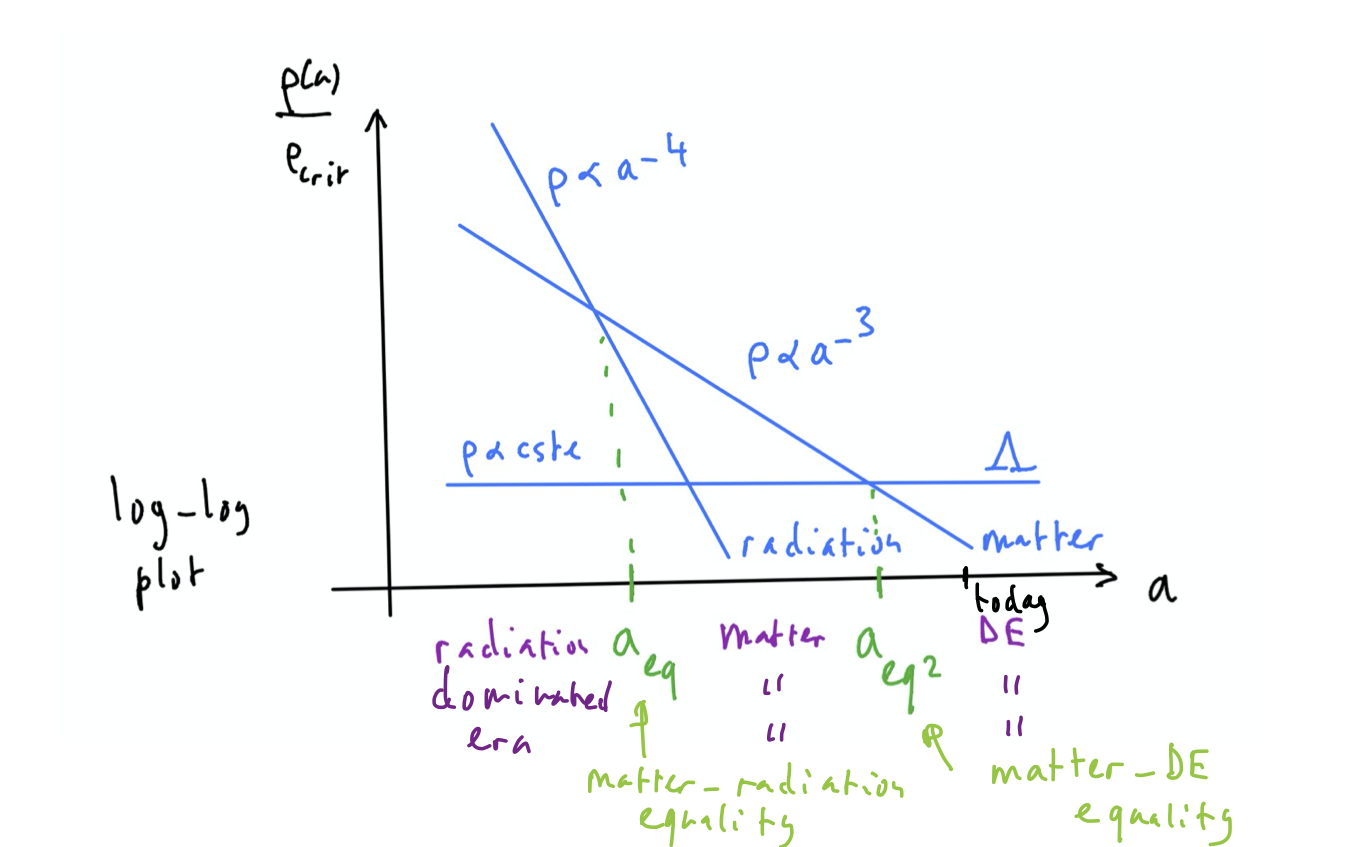
\includegraphics[width=\textwidth]{img/ch-02/domination.png}
	\caption{Domination of different components at different times}
	\label{fig:domination}
\end{figure}

\begin{table*}
\centering
\begin{tabular}{|c|c|c|c|c|}
\hline
 & $w$ & $\rho$ & $p$ & $T$\\
\hline
Matter & $0$ &  $a^{-3}$ & $a^{-5}$ & $a^{-2}$\\
\hline
Radiation & $1/3$ & $a^{-4}$ & $a^{-4}$ & $a^{-1}$\\
\hline
Radiation & $-1$ & $a^{0}$ & $a^{0}$ & -\\
\hline
\end{tabular}
\end{table*}

The results can be plugged into the Friedmann equation:
\begin{align*}
	\frac{H}{H_0} 
	&= \sqrt{\frac{\rho}{\rho_{\text{crit}, 0}} + \Omega_{K,0} \left( \frac{a_0}{a} \right)^2 }\\
	&= \sqrt{
		\Omega_{m,0} \left( \frac{a_0}{a} \right)^3
		+ \Omega_{r,0} \left( \frac{a_0}{a} \right)^4
		+ \Omega_{\Lambda,0}
		+ \Omega_{K,0} \left( \frac{a_0}{a} \right)^2
	}
\end{align*}
This is a differential equation with $\Omega_{i,0}$ as parameters.

The standard cosmological model:
\begin{itemize}
	\item $\Omega_{m,0} \approx 0.3$
	\item $\Omega_{r,0} \approx 10^{-5}$
	\item $\Omega_{\Lambda,0} \approx 0.7$
	\item $\Omega_{K,0} \approx 0$
	\item $\Omega_0 \approx 1$
	\item $h \approx 0.7$
\end{itemize}

At different times, the universe is dominated by different components. To get solutions to the Friedmann equations only the dominating component is considered:
\begin{itemize}
	\item Matter dominated:
	\begin{align*}
		\frac{H}{H_0} = \sqrt{\Omega_{m,0} \left( \frac{a_0}{a}\right)^3}
		\implies a \propto t^{2/3}
	\end{align*}
	\item Radiation dominated:
	\begin{align*}
		\frac{H}{H_0} = \sqrt{\Omega_{r,0} \left( \frac{a_0}{a} \right)^4}
		\implies a \propto t^{1/2}
	\end{align*}
	\item $\Lambda$ dominated:
	\begin{align*}
		\frac{H}{H_0} \propto \text{constant}
		\implies a \propto e^{H t}
	\end{align*}
	\item General fluid $(w \neq -1)$:
	\begin{align*}
		\rho \propto a^{-3(1+w)} \implies a \propto t^{\frac{2}{3(1+w)}}
	\end{align*}
\end{itemize}

\begin{figure}
	\centering
	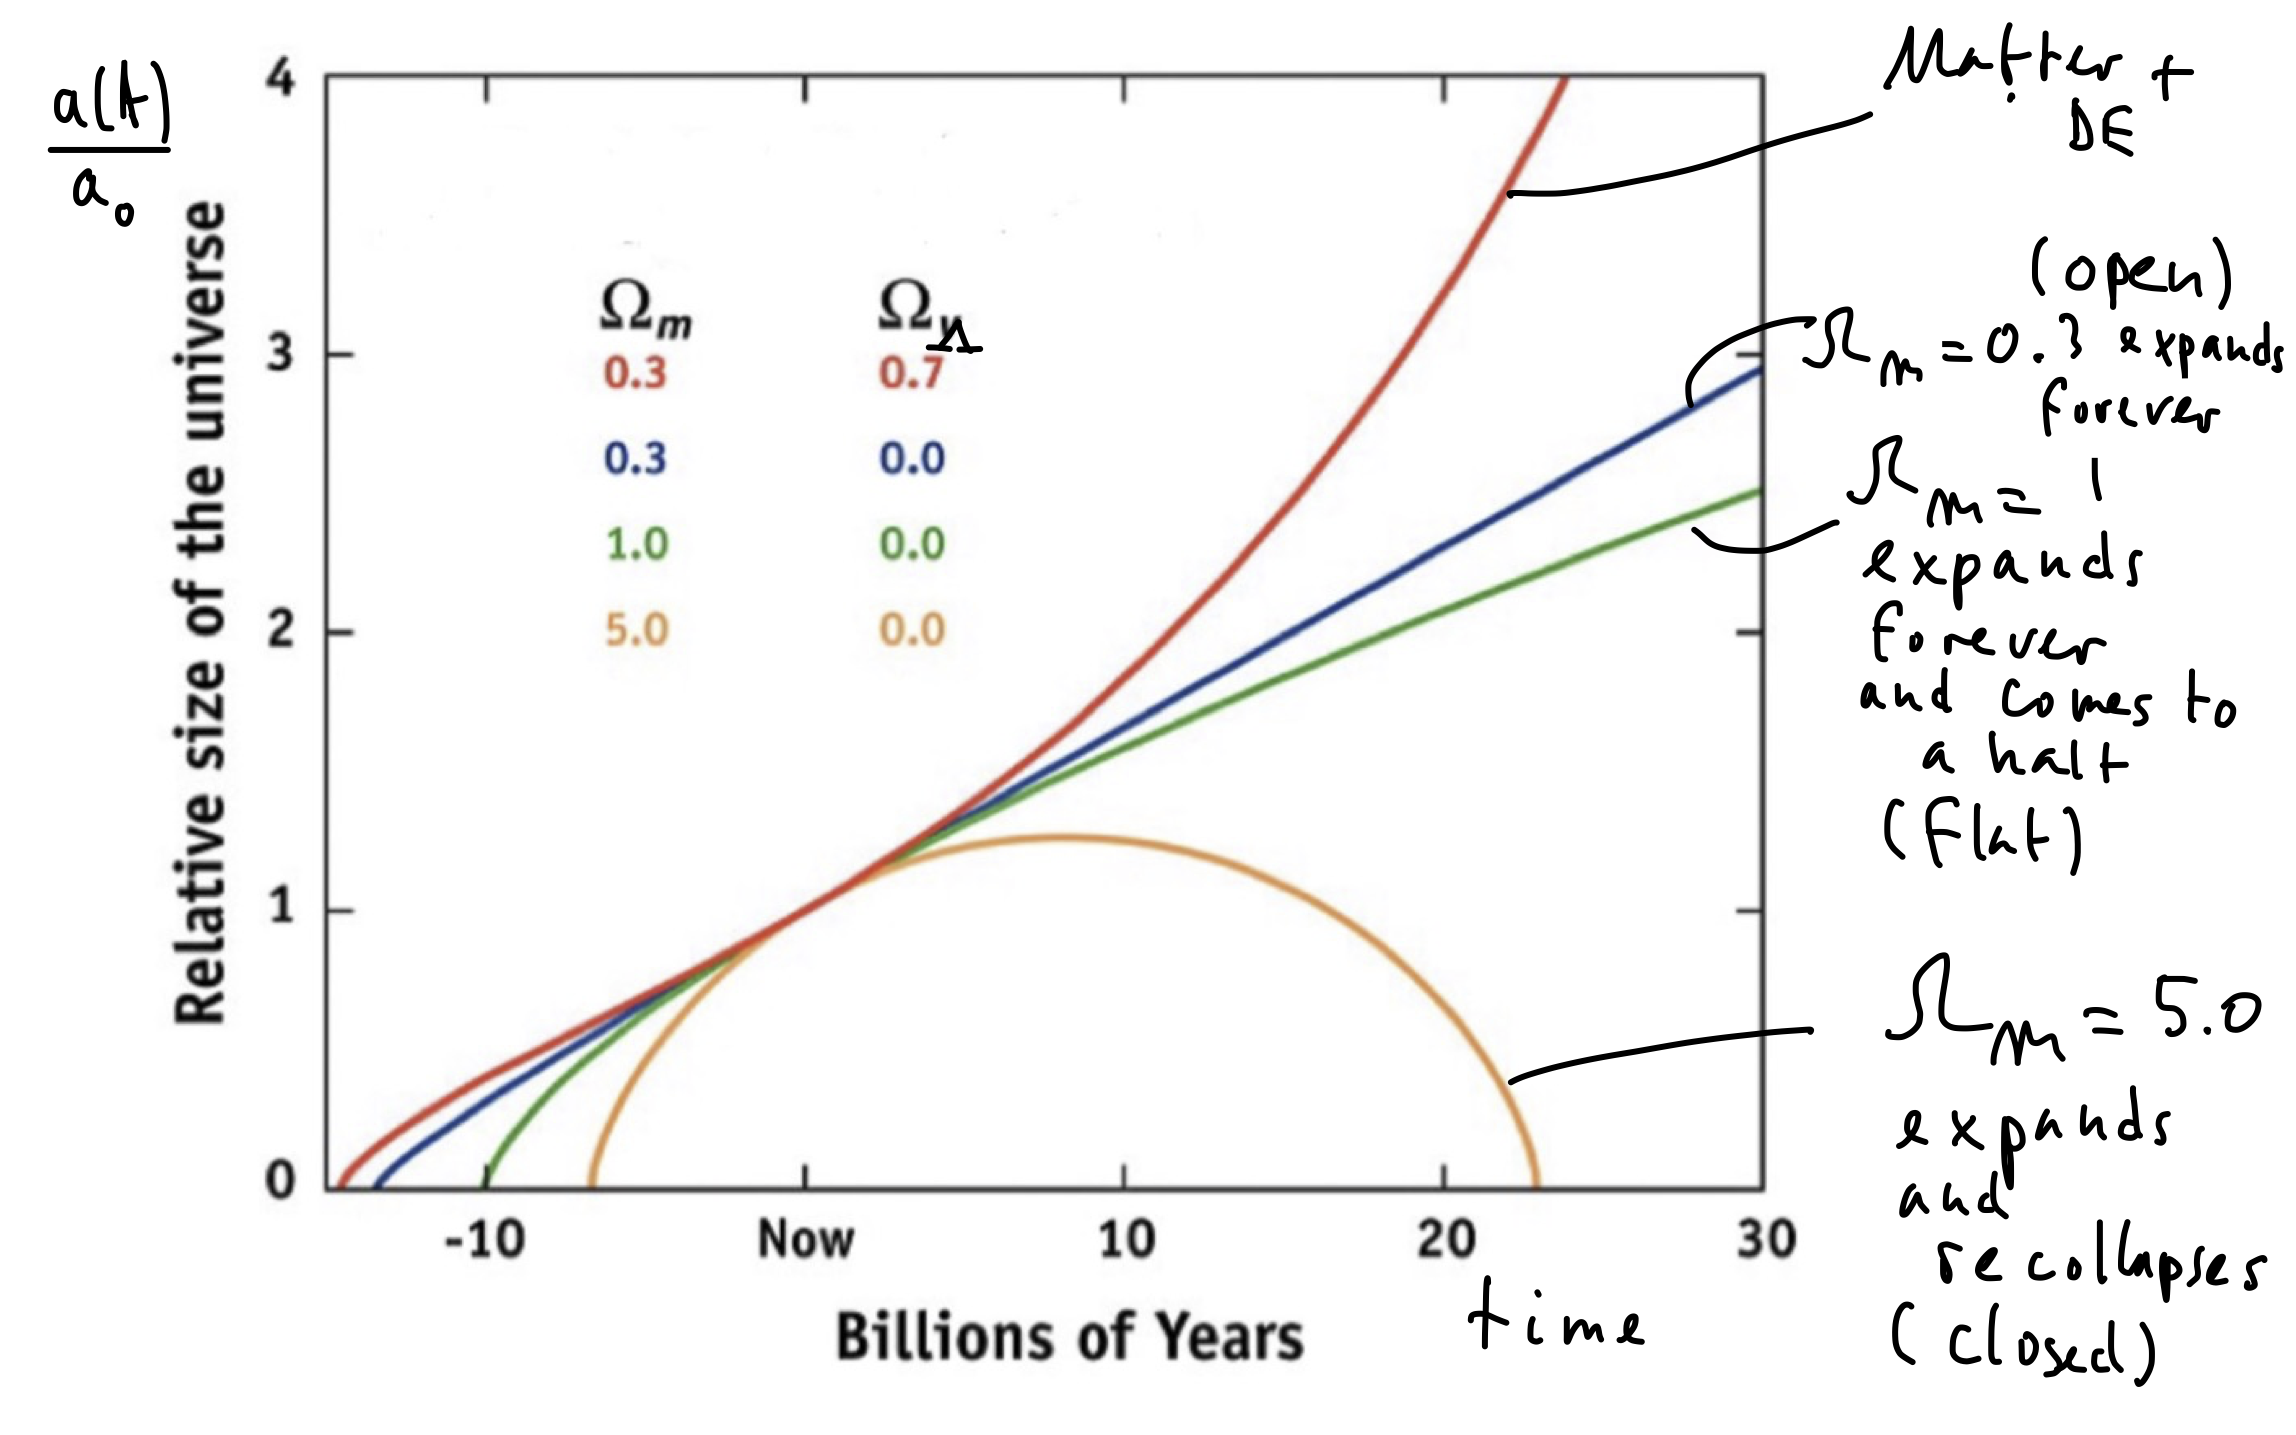
\includegraphics[width=\textwidth]{img/ch-02/evolution.png}
	\caption{Possible evolution of the universe for different density parameters.}
	\label{fig:evolution}
\end{figure}




\section{Distances and times}



\subsection{Comoving radius}
We measured the redshift of a photon that has travelled to us on a radial trajectory. How far away (in comoving distance) is the source?
\begin{align*}
	0 &= \dd{s}^2 &&\text{photon}\\
	&= c \dd{t}^2 - a(t)^2 [\dd{\chi}^2 + r(\chi)^2 \dd{\Omega}^2] &&\text{FRW metric}\\
	\implies c \dd{t} &= a(t) \dd{\chi} &&\dd{\Omega}^2 = 0 \text{ on a radial trajectory}\\
	\implies \dd{\chi} &= \frac{c \dd{t}}{a(t)}\\
	&= \frac{c \dd{a}}{a^2 H(a)} && H = \frac{\dot{a}}{a} \text{, so } \dd{t} = \frac{\dd{a}}{a H(a)}\\
	\implies \chi(a) &= c \int_a^{a_0} \frac{\dd{a'}}{a'^2 H(a')} && \chi(a_0) = 0
\end{align*}
$H(a)$ has to be obtained from the Friedmann equations. As a result, we will get $\chi(a,a_0)$. We can use $a/a_0 = 1/(1+z)$ to get $\chi(z,a_0)$. Since $a_0$ can be defined arbitrarily (for example, $a_0=1$), we get $\chi(z)$.

\subsection{Angular distance \& Luminosity distance}

The comoving distance $\chi$ and the proper distance $a \chi$ to a source are not directly observable. However, the angular size $\theta$ and the flux $F$ of an object can be measured directly.

Intrinsic properties of the source:
\begin{itemize}
	\item its size $D$
	\item its luminosity $L$
\end{itemize}
Properties of space-time:
\begin{itemize}
	\item the comoving distance to the source $\chi$
	\item the proper distance to the source $a(t) \chi$
\end{itemize}
Measurable quantities for an observer:
\begin{itemize}
	\item the angular size $\theta$
	\item the flux $F$
\end{itemize}
In Euclidean space, the following relations hold:
\begin{align*}
	\theta &= \frac{D}{d}
	& F &= \frac{L}{4 \pi d^2}
\end{align*}
where $d$ is the distance to the source. In FRW-space, we define the following:
\begin{itemize}
	\item The angular-diameter distance $d_A$ satisfies $\theta = D/d_A$. One can show $d_A = a \cdot r(\chi)$, where $r(\chi) = D/(a \theta) = D_{comoving}/\theta$ is the comoving angular diameter distance.
	\item The luminosity distance $d_L$ satisfies $F = L/(4\pi d_L^2$). One can show that $d_L = a_0 r(\chi) (1+z) = d_A (1+z)^2$. Taking $a_0 = 1$ yields $d_L = r(\chi)/a = d_A/a^2$. 
\end{itemize}
In a static space $d = d_A = d_L$ would hold. 

\subsection{Comoving Horizon}
Suppose a (hypothetical, non-interacting) photon was emitted at the Big Bang. How far (in comoving distance) could it have travelled until now? This comoving distance is called the comoving horizon. We plug into the equation of the comoving radius/distance, with $a=0$ at the start:
\begin{align*}
	\chi_h
	&= \chi (r_h) = c \int_0^{a_0} \frac{\dd{a'}}{a'^2 H(a')}
\end{align*}

\subsection{Age of the Universe}
How old is the universe?
\begin{align*}
	t_0 &= \int_0^{t_0} \dd{t}\\
	&= \int_0^{a_0} \frac{\dd{a}}{a H(a)} && H(a) = \dot{a}/a
\end{align*}
$H(a)$ is again found from the Friedmann equation. With the standard cosmological model, $t_0 \approx \SI{14}{\giga\year}$.





\section{Thermal history of the Universe}
\label{sec:thermal-history}

According to the Big Bang paradigm, the universe was once hot and dense, and now it expands and cools down. Today, it is far from thermal equilibrium, but it must have been in thermal equilibrium at some point in the past if it continuously expands.

The matter content at each epoch depends on:
\begin{itemize}
	\item Thermodynamics
	\item Particle, nuclear and atomic physics
\end{itemize}

A system is in thermal equilibrium if $\Gamma \gg H$
\begin{itemize}
	\item $\Gamma = \text{interactions}/\text{time}$ is the interaction rate
	\item $H = \dot{a}/a$ is the Hubble constant
\end{itemize}
Similarly, a system is in thermal equilibrium if $\tau_\Gamma \ll \tau_H$
\begin{itemize}
	\item $\tau_\Gamma = 1/\Gamma$ is the characteristic timescale of interactions
	\item $\tau_H = 1/H$ is the characteristic timescale of expansion
\end{itemize}
We already know about $H$. $\Gamma$ is defined as
\begin{align*}
	\Gamma = n v \sigma
\end{align*}
\begin{itemize}
	\item $n \quad$ number density, $\text{particles}/\text{volume}$
	\item $v \quad$ velocity of particles
	\item $\sigma \quad$ scattering cross-section, has units of area.
\end{itemize}

At early times, $\Gamma \gg H$. Particles are in thermal equilibrium with the plasma and coupled to photons. This scenario will be treated in \cref{ssec:early-times}.

At later times $\Gamma \ll H$. Particles are not in thermal equilibrium and are decoupled from photons. See \cref{ssec:late-times}

The decoupling or \enquote{freeze out} happens when $\Gamma \approx H$. This transition is described by the Boltzmann equation in \cref{ssec:boltzmann}.

In \cref{tab:thermal-history} and \cref{fig:evolution}, an overview of the thermal history of the universe is given.

\begin{table*}
	\centering
	\tabulinesep=2mm
	\begin{tabu}{m{10cm}llp{2cm}}
	\toprule
	Event & time & redshift & energy \newline temp.\\
	\midrule
	\describe{Inflation}{A phase of extremely rapid exponential expansion, caused by a phase transitions where the inflaton field emerged. Inflation explains properties of the universe which are difficult to account for without.}
	 & $10^{-34}$ s & ? & ? \\
	\describe{Baryogenesis}{Baryons (protons, neutrons) are formed from quarks. Weirdly, there are way more baryons formed than antibaryons. This is the matter-antimatter asymmetry.} & ? & ? & ? \\
	\describe{QCD phase transition}{The universe has cooled sufficiently such that hadrons (baryons and mesons) can form.} & \SI{e-5}{\second} & \num{e12} & \SI{200}{\MeV} \newline \SI{3e12}{\kelvin}\\
	Pions annihilate and decay, the only hadrons left are nucleons (protons and neutrons). & \SI{e-4}{\second} &  & \SI{50}{\MeV} \newline \SI{e12}{\kelvin}\\
	\describe{Dark Matter freeze-out}{Dark Matter interacts very weakly with ordinary matter, so it decouples early on.} & ? & ? & ?\\
	\describe{Electron-positron annihilation}{Electrons and positrons annihilate through $e^+ + e^- \to 2 \gamma$. Since the number of charged particles decreases, neutrinos decouple. The n/p ratio freezes out at $n_n \approx 1/10 n_p$.} & \SI{4}{\second} & \num{2e9} & \SI{0.3}{\MeV} \newline \SI{5e9}{\kelvin}\\
	\describe{Big Bang nucleosynthesis}{Light nuclei such as D and He get synthesized. They are still ionized.} & \SI{3}{\minute} & \num{4e8} & \SI{0.08}{\MeV} \newline \SI{e9}{\kelvin}\\
	\describe{Matter-radiation equality}{} & \SI{6e4}{\year} & \num{3400} & \SI{0.75}{\eV} \newline \SI{8700}{\kelvin}\\
	\describe{Recombination}{Formation of neutral atoms through $e^- + p^+ \to H + \gamma$} & \SI{2e5}{\year} & \num{1200} & \SI{0.34}{\eV} \newline \SI{4000}{\kelvin}\\
	\describe{Surface of last scattering}{The number density of charged particles has decreased enough for photons to decouple. These photons form the CMB.} &  &  & \\
	\describe{Reionization}{Stars form and re-ionize neutral hydrogen.} & \SI{2e8}{\year} & \num{20} & \SI{4}{\meV} \newline \SI{50}{\kelvin}\\
	\describe{Dark Energy - Matter equality}{} & \SI{9}{\giga\year} & \num{0.4} & \SI{0.33}{\meV} \newline \SI{3.8}{\kelvin}\\
	\describe{Today}{} & \SI{13.8}{\giga\year} & \num{0} & \SI{0.24}{\eV} \newline \SI{2.7}{\kelvin}\\
	\bottomrule
	\end{tabu}
	\caption{Thermal history of the universe}
	\label{tab:thermal-history}
\end{table*}

\begin{figure}
	\centering
	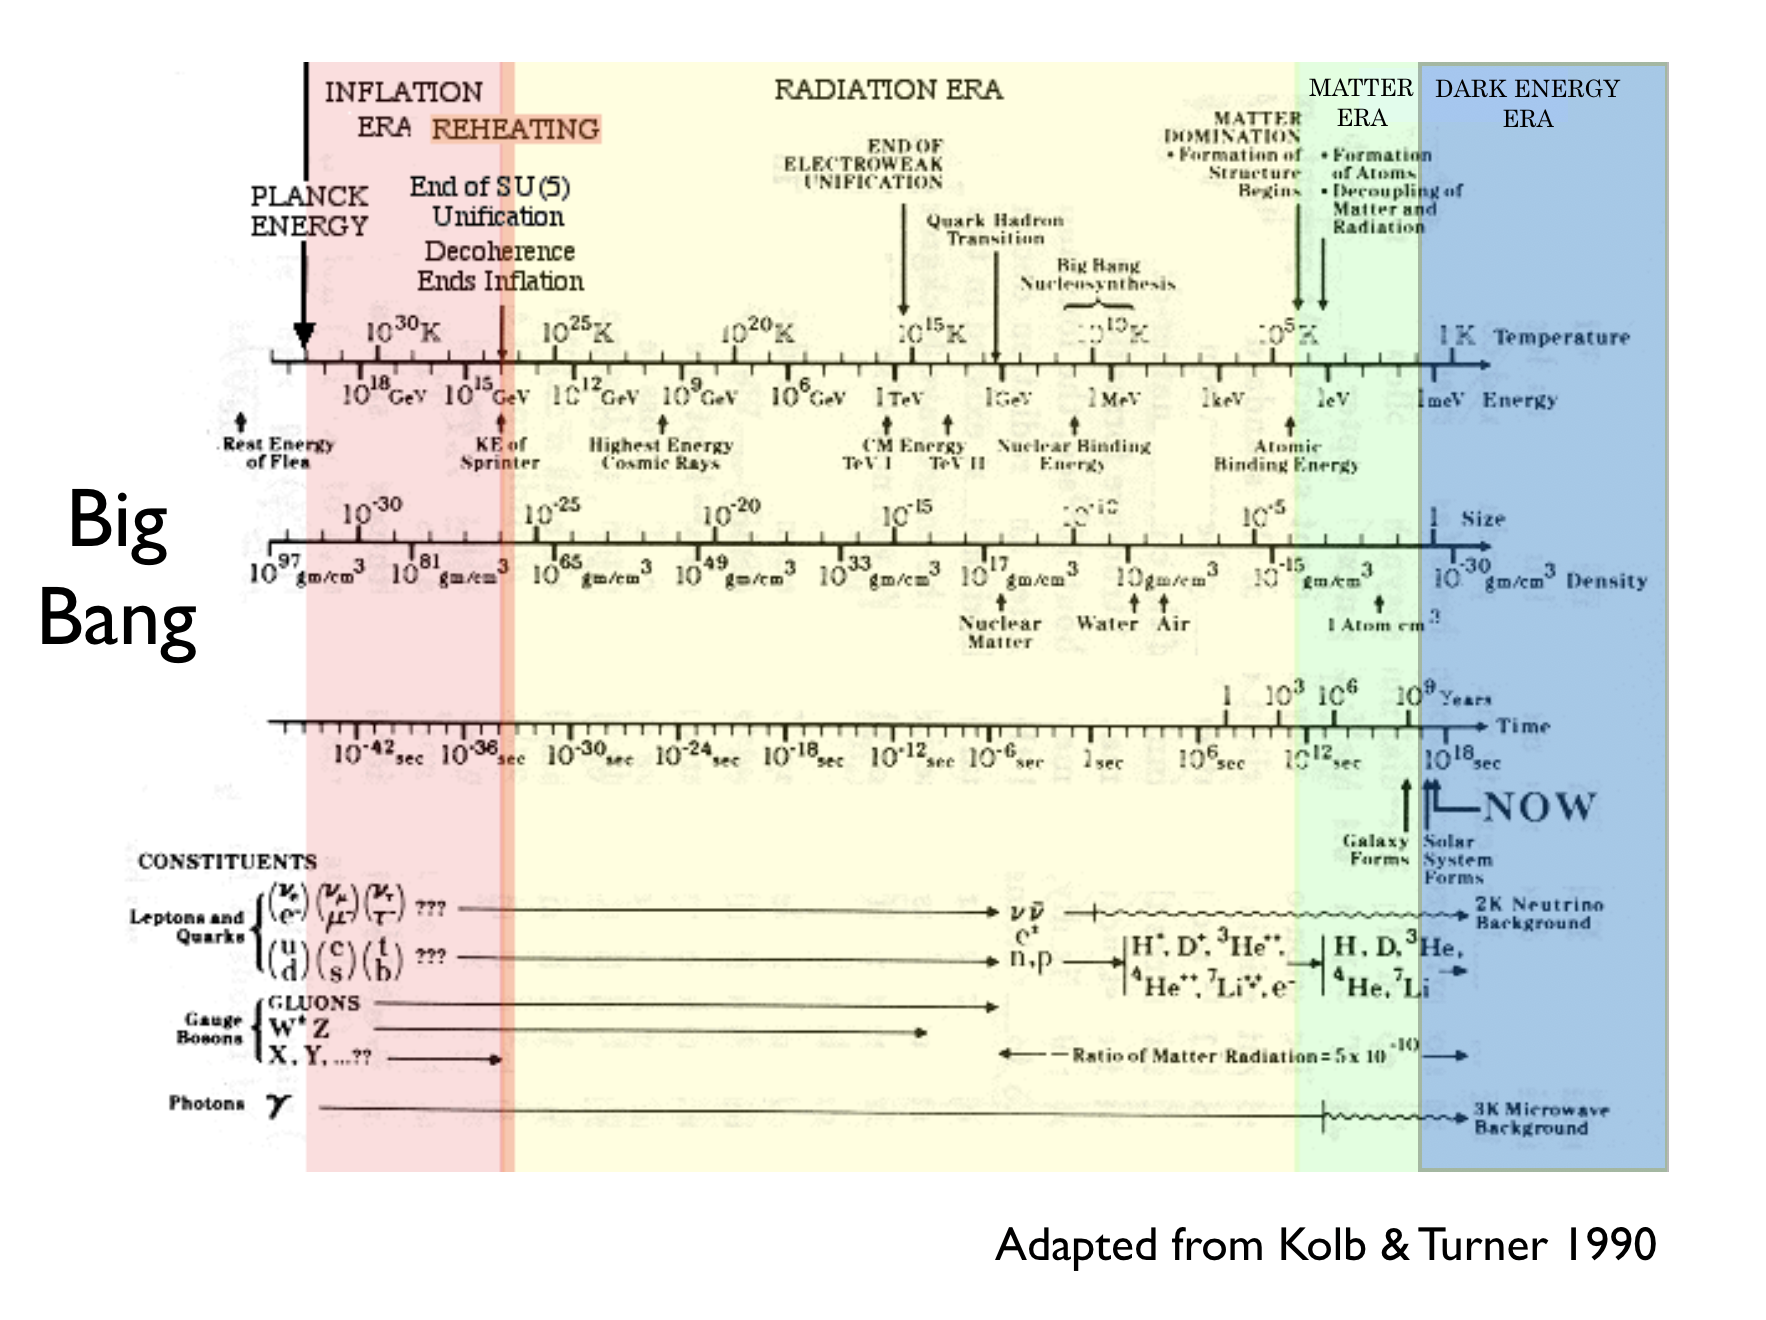
\includegraphics[width=\textwidth]{img/ch-02/big-bang.png}
	\caption{History of the Big Bang}
	\label{fig:big-bang}
\end{figure}

\section{Thermodynamics in an expanding Universe}

To describe the evolution of the universe quantitatively, a few definitions are required:

\begin{itemize}
	\item The probability that a particle at time $t$ is in a volume $\dd{^3 x} \dd{^3 p}$ around ($ \vec{x}, \vec{p}$) is given by the \textbf{(phase space) distribution function}:
	\begin{align*}
		f(\vec{x}, \vec{p}, t) \dd{^3 x} \dd{^3 p}
	\end{align*}
	In a homogeneous and isotropic universe, we have $f(\vec{x}, \vec{p}, t) = f(p, t)$.
	\item The number of particles per unit volume is given by the \textbf{number density}:
	\begin{align*}
		n(t) = 4\pi \int f(p,t) p^2  \dd{p}
	\end{align*}
	\item The energy per unit volume is given by the \textbf{energy density}:
	\begin{align*}
		\rho(t) = 4 \pi \int E(p) f(p,t) p^2 \dd{p},
	\end{align*}
	with $E(p) = \sqrt{p^2 + m^2}$  (natural units are used, therefore $c= k_B = \hbar = 1$).
	\item The \textbf{pressure} is given by
	\begin{align*}
		P(t) = 4 \pi c^2 \int \frac{p^2}{3 E(p)} f(p,t) p^2 \dd{p}
	\end{align*}
	Since we work in natural units, we drop the $c$.
\end{itemize}


\subsection{At early times ($\Gamma > H$)}
\label{ssec:early-times}
The distribution function of particles in thermodynamic equilibrium is the Bose-Einstein (bosons) or the Fermi-Dirac (fermions) distribution:
\begin{align*}
	f_\text{eq}(p,t)
	= \frac{g}{(2\pi)^3} \left[ \exp\left( 
		\frac{E(p)-\mu}{T} \pm 1
	 \right) \right]^{-1}
\end{align*}
\begin{itemize}
	\item $+$ is for fermions and $-$ for bosons
	\item $g$ is a spin degeneracy factor. Examples: $g_\nu = 1$, $g_\gamma = 2$, $g_\text{quark} = 6$
	\item $\mu$ is the chemical potential, which is the response of a thermodynamical system to a change of particle number. Usually, $\mu=0$ for our purposes.
	\item $T$ is the temperature of the universe at time t.
\end{itemize}

For \emph{non-relativistic particles}, $T \ll m$ and $E \approx m + p^2/2m$. Plugging this in yields
\begin{align*}
	n_{eq} &= g \left( \frac{m T}{2 \pi} \right)^{3/2} \exp\left( \frac{\mu-m}{T} \right)&
	\rho_{eq} &= n m&
	P_{eq} &= n T
\end{align*}
Note that the pressure equation is identical to the ideal gas equation in natural units. 

For \emph{relativistic particles}, $T \gg m$ and $E \approx p$. For both fermions and bosons, this yields
\begin{align*}
	n_{eq} &\propto g T^3&
	\rho_{eq} &\propto g T^4&
	P_{eq} &= \frac{\rho_{eq}}{3}
\end{align*}
Note that the pressure equation is identical to the equation of state as seen in \cref{sec:Friedmann}.
In the case of a relativistic gas, $T \propto a^{-1}$, so $n \propto a^{-3}$ and $\rho \propto a^{-4}$. This is what we have already seen in \cref{sec:Friedmann}.


% \begin{tabular}{lccc}
% \toprule
% & $n$ & $\rho$ & $P$\\
% \midrule
% non-relativistic particle & $g \left( \frac{m T}{2 \pi} \right)^{3/2} \exp\left( \frac{p-m}{T} \right)$ & $n m$ & $n T$\\
% relativistic particle & $gT^3$ & $gT^4$ & $\rho/3$\\
% relativistic gas & $g a^{-3}$ & $g a^{-4}$ & \\
% \bottomrule
% \end{tabular}


\subsection{At late times ($\Gamma < H$)}
\label{ssec:late-times}
The transition between non-equilibrium and equilibrium takes place at the decoupling time of freeze-out time $t_f$, where $T \approx T_f = T_{\gamma}(t_f)$. At $t>t_f$, the distribution function is
\begin{align*}
	f(p,t) = f\left( p \frac{a(t)}{a(t_f)}, t_f \right)
\end{align*}
The shape of the function is \enquote{frozen in} at the freeze-out time $t_f$.

For a relativistic particle,
\begin{align*}
	f(p,t) =
	 \frac{g}{(2\pi)^3} \left[ \exp\left( 
		\frac{p a(t)}{T_f a(t_f)} \pm 1
	 	\right) \right]^{-1},
\end{align*}
which is the same as for an equilibrium particle, but with $T_f \defeq T_f a(t_f)/a(t)$.



\subsection{Boltzmann equation}
\label{ssec:boltzmann}
The Boltzmann equation
\begin{align*}
	\dv{f_i}{t} = C_i[f]
\end{align*}
describes the time evolution of the distribution function between early and late times. $C_i[f]$ is the collision term, which describes the change of $f_i$ due to interactions with other species.

$f_i$ only depends on $p$ and $t$, so we can write
\begin{align*}
	\dv{f_i}{t} &= \pdv{f_i}{t} + \pdv{f_i}{p} \dv{p}{t}
\end{align*}
The last term can be simplified. Because $p = p_0 a^{-1}$, $\dv*{p}{t} = -p_0 a^{-2} \dot{a} = - p H$. The Boltzmann equation for a homogeneous and isotropic case then becomes
\begin{align*}
	\pdv{f_i}{t} - p H(t) \pdv{f_i}{p} &= C_i[f]\\
	\implies \pdv{}{t} \int \dd{^3 p} f_i - H(t) \int \dd{^3 p} p \pdv{f_i}{p} &= \int \dd{^3 p} C_i[f]\\
	\implies \dv{n_i}{t} + 3 H(t) n_i &= \int \dd{^3 p} C_i[f]
\end{align*}
In the last line, we used partial integration.\sidenote{In detail:
\begin{align*}
	\int \dd{^3p} p \pdv{f_i}{p}
	&= \int \dd{p} p^3 \pdv{f_i}{p}\\
	&= - \int \dd{p} \pdv{p^3}{p} f_i \\
	&= -3 n_i
\end{align*}}
If the system is collisionless, $C_i[f]=0$, and the solution of the Boltzmann equation is $n_i \propto a^{-3}$ as expected. The $3H(t) n_i$ is called the Hubble drag term.

We now look at reactions of the type $i + j \leftrightarrow a + b$. The collision term is then of the form
\begin{align*}
	C_i[f] = \alpha(T) n_a n_b - \beta(T) n_i n_j
\end{align*}
\begin{itemize}
	\item $\alpha(T)$ is the production rate
	\item $\beta(T)$ is the destruction rate
\end{itemize}
If we insert this collision term into the equation we get
\begin{align*}
	\dv{n_i}{t} + 3 H(t) n_i = \alpha(T) n_a n_b - \beta(T) n_i n_j. 
\end{align*}
Writing the same equation for the species j and combine these two equations, one finds that
\begin{align*}
	(n_i - n_j)a^3 = \text{constant}. 
\end{align*}
To simplify the collision term of the equation, we make a few assumptions:
\begin{itemize}
	\item species $a$ and $b$ are in equilibrium with a general hot plasma at temperature $T = T_a = T_b$
	\item $n_i = n_j$ (e.g. in the case of antiparticles)
	\item radiation era: $a \propto t^{1/2} \propto T^{-1}$
\end{itemize}
The equation then becomes
\begin{align*}
	\dv{n_i}{t} + 3 H(t) n_i = \beta(T) (n_{i, \text{eq}}^2 - n_i^2), 
\end{align*}
where $n_{i, \text{eq}}$ is the equilibrium density for i. 
To analyse the equation, we define
\begin{itemize}
	\item $x = m_i/T$ is used as a time variable
	\item $Y_i = n_i/s$, where $s \propto a^{-3}$ is the entropy
	\item $\Gamma(x) = n_{i, \text{eq}}(x) \beta(x)$
\end{itemize}
One finally gets a differential equation for $Y_i(x)$
\begin{align*}
	\frac{x}{Y_{i, \text{eq}}} \dv{Y_i}{x} = - \frac{\Gamma(x)}{H(x)} \left[ \left( \frac{Y_i}{Y_{i,\text{eq}}} \right)^2 - 1 \right]
\end{align*}
with initial condition: $x \ll 1$ at early times, so $Y_i = Y_{i, \text{eq}}$.

No analytical solution is known. A set of numerical solutions is shown in \cref{fig:boltzmann}

\begin{marginfigure}
	\centering
	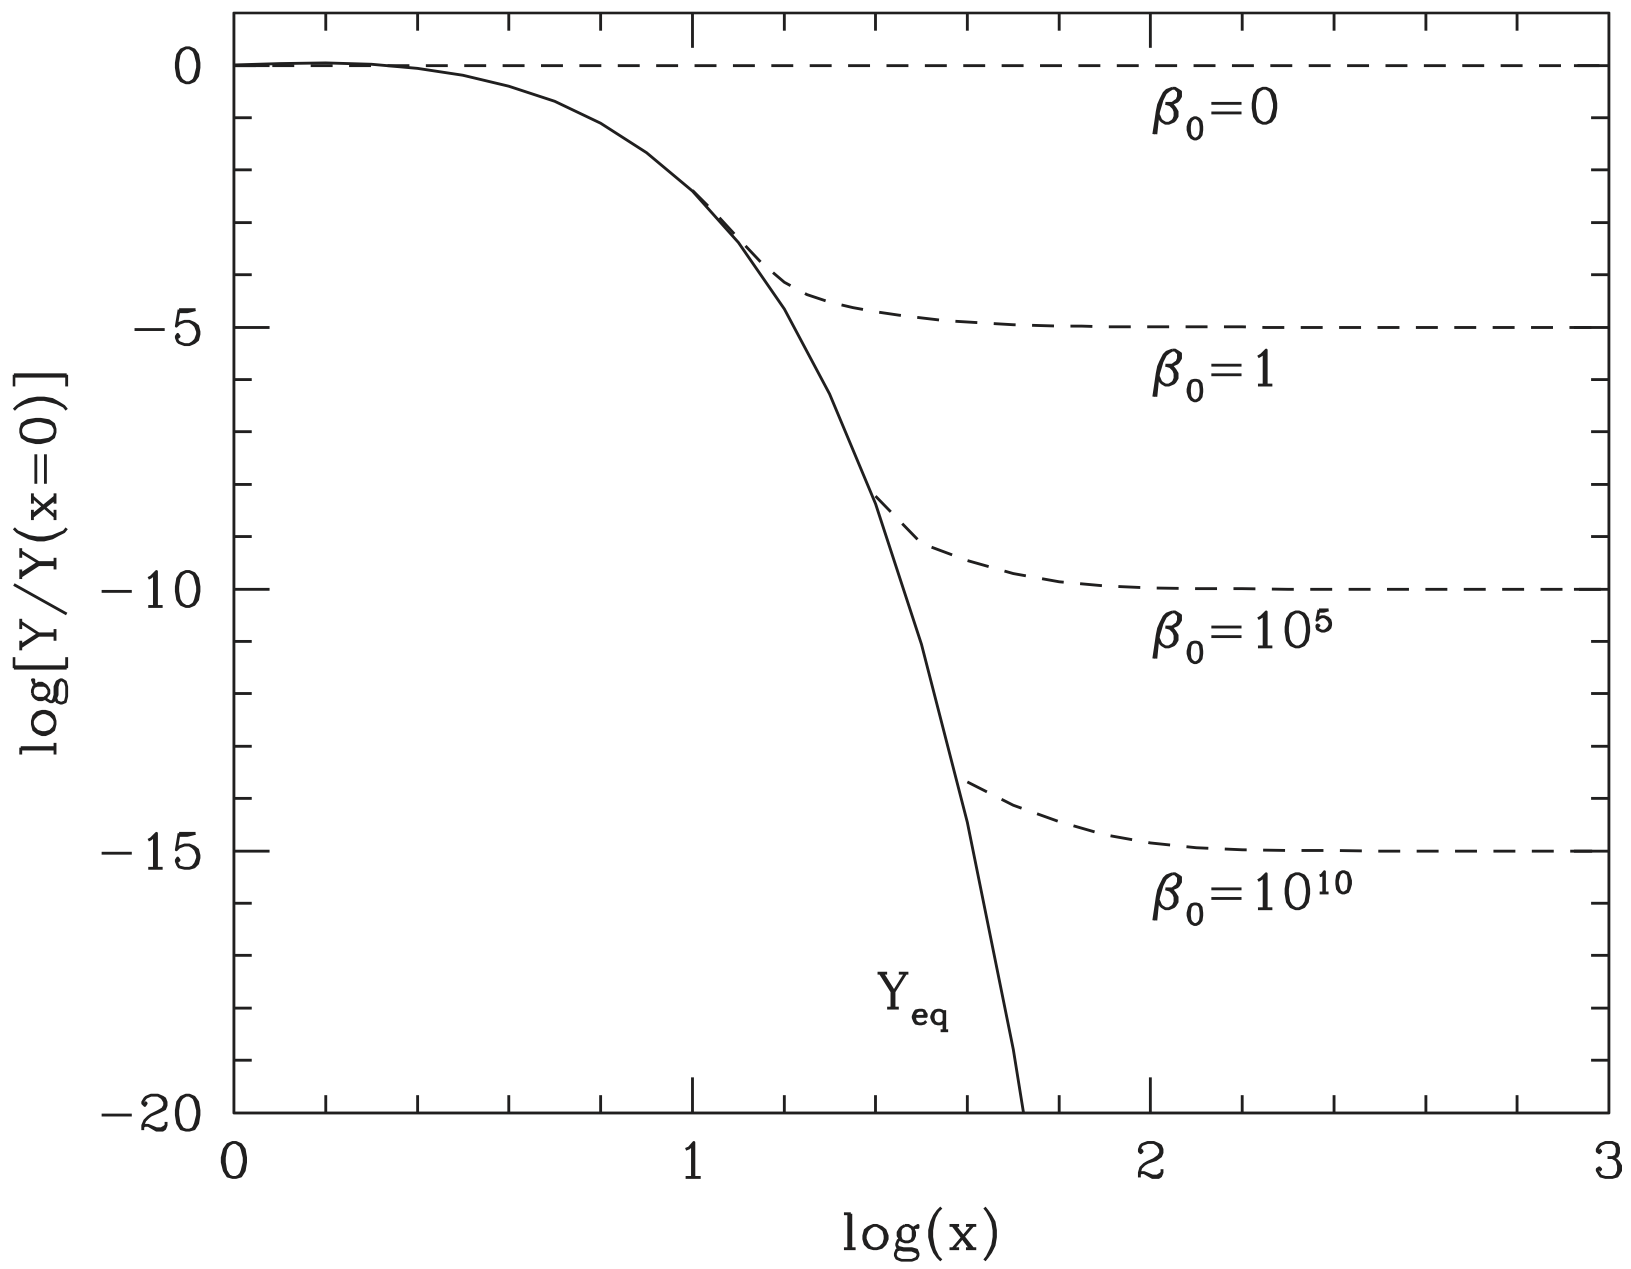
\includegraphics[width=\textwidth]{img/ch-02/boltzmann.png}
	\caption{Solutions of the Boltzmann equation for different destruction rates $\beta$. We assume $\beta(T) = \beta_0$ is constant. The vertical axis is a proxy for abundance, and the horizontal axis for time. First, particles remain in equilibrium (solid line), then they decouple (dashed lines), leaving relic abundances. When $\beta_0$ is large, thermal equilibrium is maintained longer, so the relic abundance is lower.}
	\label{fig:boltzmann}
\end{marginfigure}


\section{Particle relics}
There are two types of relics:
\begin{itemize}
	\item Hot relics freeze out when the particles are still relativistic. Since $x = m_i / T$, this means $x_f \ll 1$
	\item Cold relics freeze out when the particles are already non-relativistic, with $x_f \gg 1$
\end{itemize}

\subsection{Hot relics}
We consider now only those relics that are still relativistic today, with rest mass $m_i \ll T_0 = \SI{2.4e-4}{\eV}$. An example would be massless neutrinos.

The solution of the Boltzmann equation is
	\begin{align*}
		\Omega_{i,0} h^2
		&= \frac{ g_{i,\text{eff}} }{2}  \left[ \frac{g_{*s}(x_0)}{g_{*s}(x_f)} \right]^{4/3} \Omega_{\gamma, 0} h^2
	\end{align*}
The $g$'s are degeneracy factors and satisfy $g_{*s}(x_0) \leq g_{*s}(x_f)$, and the photon density is $\Omega_{\gamma,0} h^2 = \num{2.5e-5}$. It follows that $\Omega_{i,0}$ is very small, which means that hot relic particles contribute very little to today's energy density.

\subsection{WIMPs}
Next we consider weakly interacting massive particles (WIMPs). Examples are massive neutrinos and stable, light supersymmetric particles. WIMPs can either be hot ($x_f \ll 1$) or cold ($x_f \gg 1$).

\paragraph*{Hot WIMPs}
The solution of the Boltzmann equation yields
\begin{align*}
	\Omega_{i,0} h^2 = \num{7.64e-2} 
	\left( \frac{g_{i,\text{eff}}}{g_{*s}(x_f)} \right)
	\frac{m_i}{\si{\eV}}
\end{align*}
Since we know that $\Omega_{i,0} < 1$, we can get a constraint $m_i < \SI{94}{\eV}$ on the mass of the hot WIMPs, which is possible for neutrinos. However, hot WIMPs are ruled out as dark matter by structure formation arguments.

\paragraph*{Cold WIMPs}
Boltzmann says
\begin{align*}
	\Omega_{i,0} h^2
	&= \begin{cases}
	1.8 \left( \frac{m_i}{\si{\GeV}} \right)^{-2} 
	\left[ 1 + 0.17 \ln\left( \frac{m_i}{\si{\GeV}} \right) \right]
	& \text{if } m_i < \SI{100}{\GeV}\\
	\left( \frac{m_i}{\SI{3}{\TeV}} \right)^2
	& \text{if } m_i > \SI{100}{\GeV}
	\end{cases}
\end{align*}
To get $\Omega_{i,0} < 1$, we need $m_i$ to be between $\SI{1.4}{\GeV}$ and $\SI{3}{\TeV}$. Cold Wimps are good candidates for dark matter.

\section{Primordial nucleosynthesis}

This is the epoch where protons and neutrons first combined to nuclei (not atoms) heavier than hydrogen. Heavier atoms can also be synthesized in stars through nuclear reactions, which has to be differentiated in observations.

\subsection*{Initial conditions}

Initially, the temperature is $T < \SI{e13}{\kelvin}$ and the associated energy scale is $k_B T \approx \SI{0.8}{\MeV}$. Protons and neutrons are in thermal equilibrium and interact weakly via the processes $p + e \leftrightarrow n + \nu_e$ and $n + \bar{e} \leftrightarrow p + \bar{\nu}_e$. Since the mass of the nucleons is around \SI{940}{\MeV}, they are already non-relativistic. The masses of neutrons and protons are slightly different, so their abundances after freeze out are different.

\subsection*{Nuclear reactions}

Once the temperature drops below \SI{1}{\MeV}, which is the binding energy of a typical nucleus, the nuclei start forming. A host of nuclear reactions can occur then:
\begin{align*}
	\ce{p + n &<=> \gamma{} + D} &
	\ce{D + n &<=> \gamma{} + ^3H} \\
	\ce{D + D &<=> p + ^3H} &
	\ce{D + p &<=> \gamma{} + ^3He} \\
	\ce{D + D &<=> n + ^3He} &
	\ce{^3H + p &<=> n + ^3He} \\
	\ce{^3H &<=> e + \bar{\nu}_e + ^3He} &
	\ce{^3H + p &<=> \gamma{} + ^4He} \\
	\ce{^3H + D &<=> n + ^4He} & 
	\ce{^3He + n &<=> \gamma{} + ^4He} \\
	\ce{^3He + D &<=> p + ^4He} &
	\ce{2 ^3He &<=> 2p + ^4He} \\
	\ce{^7Li + p &<=> 2 ^4He} &
	\ce{^4He + ^3H &<=> \gamma{} + ^7Li} \\
	\ce{^4He + ^3He &<=> \gamma{} + ^7Be} &
	\ce{^7Be + e &<=> \nu_e + ^7Li}
\end{align*}
For each of these reactions, there is a Boltzmann equation which describes the evolution of the number densities. This coupled system of equations can be solved numerically to find the abundances of nuclei. The solution for a few nuclei is shown in \cref{fig:nucleosynthesis}.


\begin{marginfigure}
	\centering
	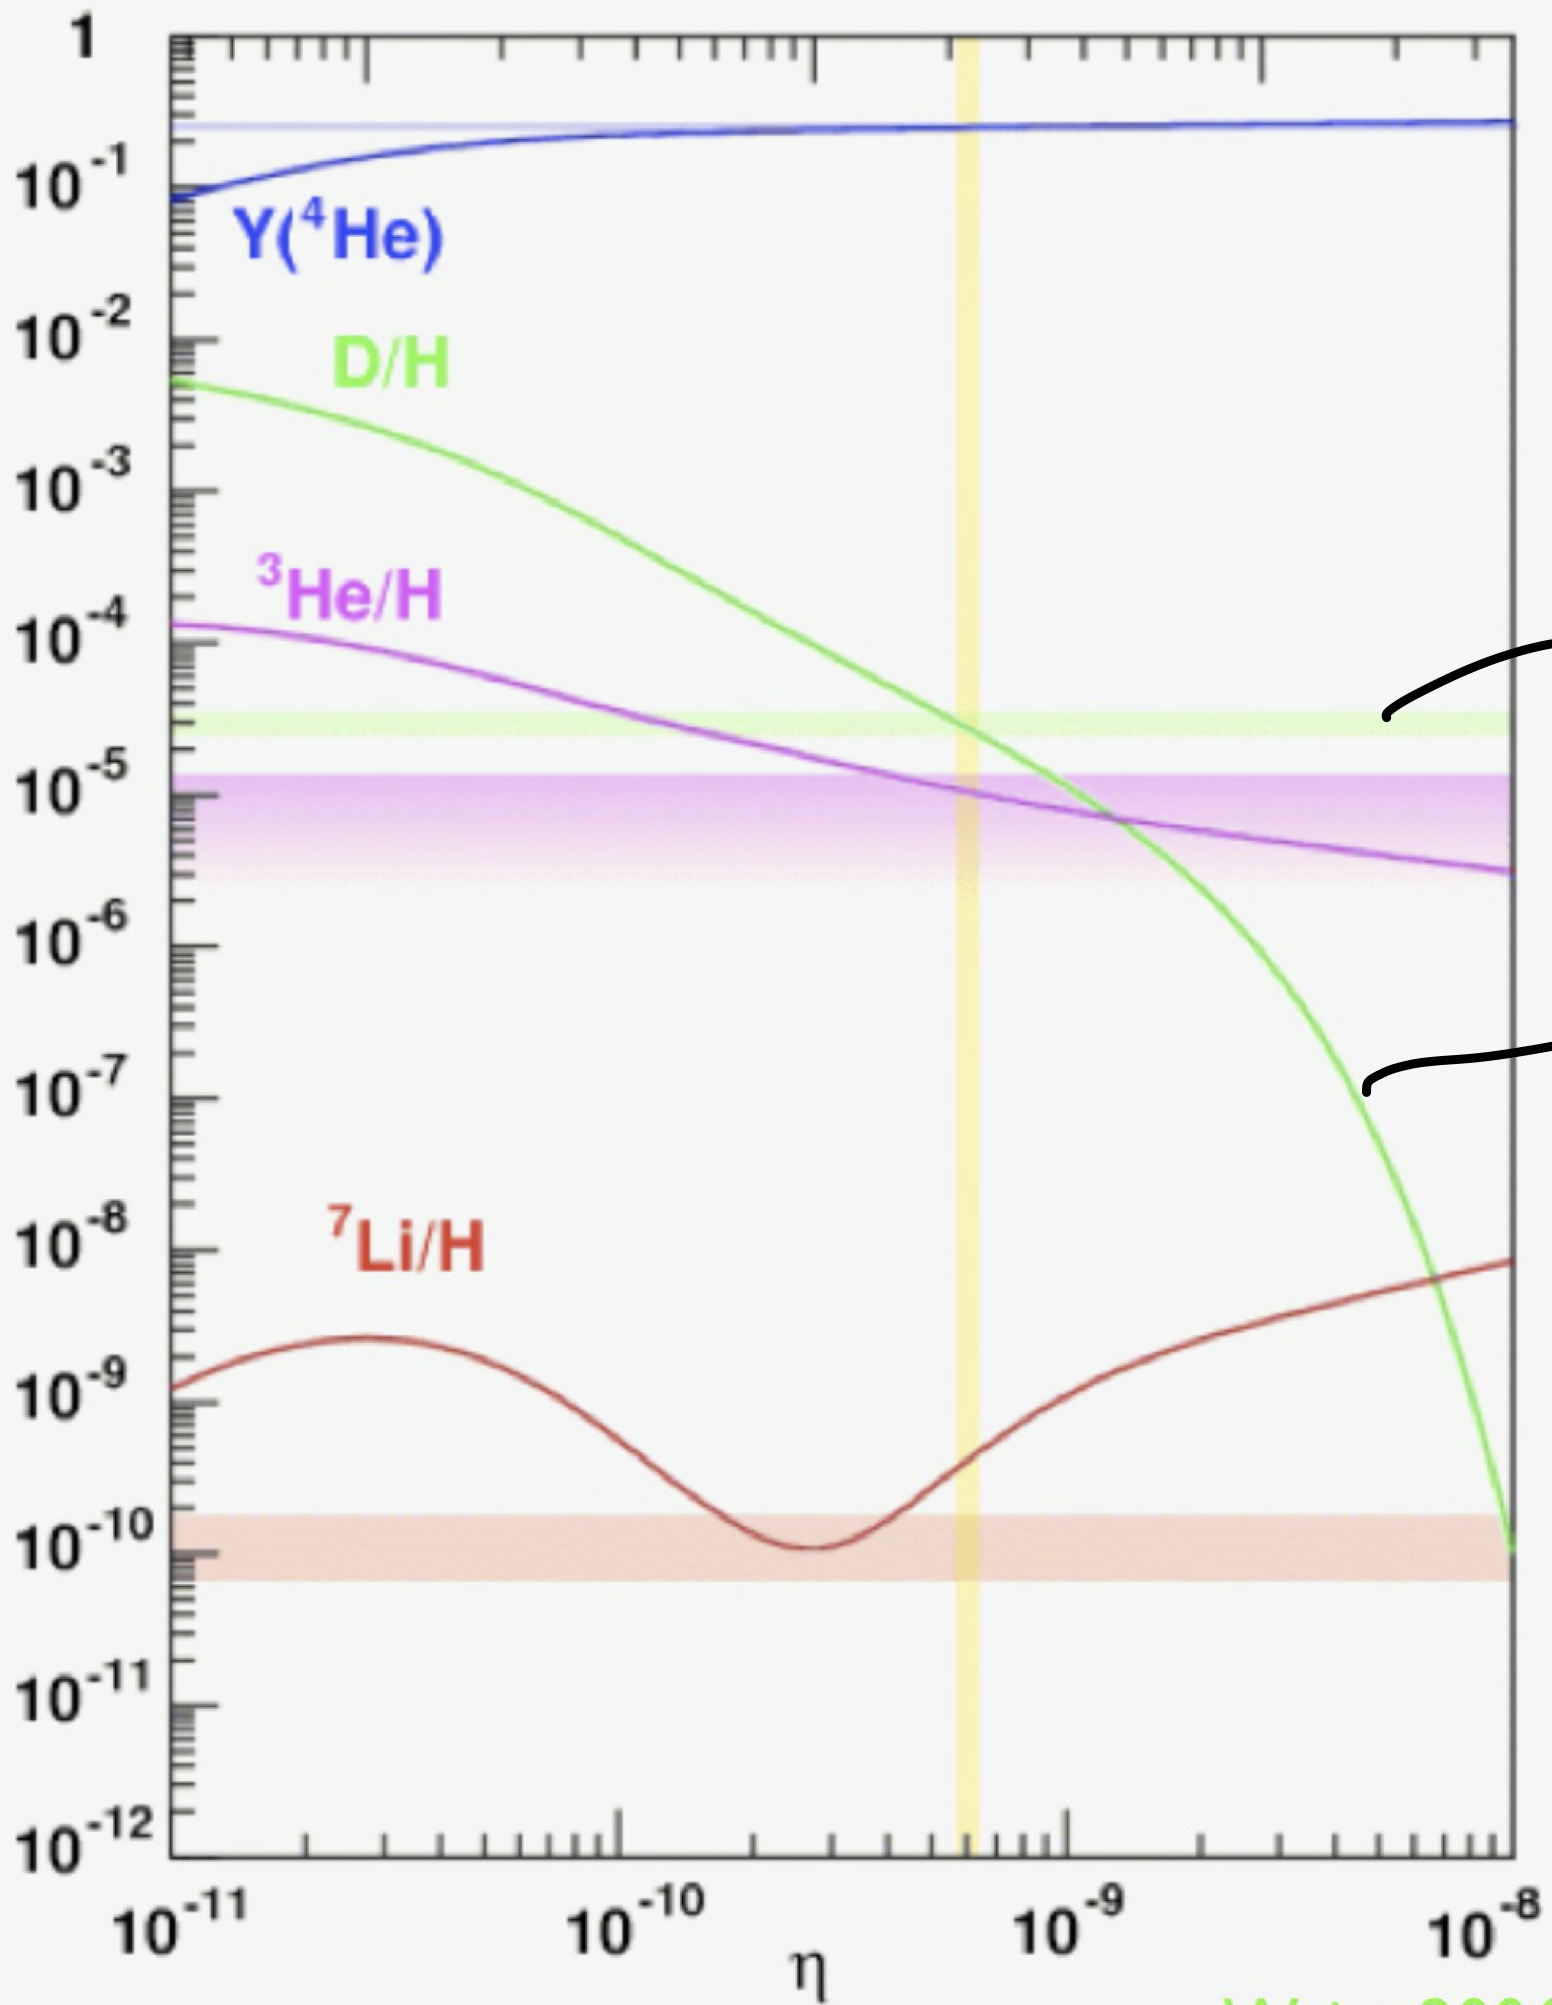
\includegraphics[width=\textwidth]{img/ch-02/nucleosynthesis.png}
	\caption{The abundances of \ce{D}, \ce{^4He}, \ce{^3He}, and \ce{^7Li}, as a function of the photon to baryon ration $\eta$. The yellow vertical area indicates the measured value of $\eta$, while the shaded horizontal bars are the measured abundances. The modelled abundances agree well with the experiments, except for \ce{^7Li}, which is probably due to uncertainties in how much \ce{^7Li} is destroyed in stars.}
	\label{fig:nucleosynthesis}
\end{marginfigure}


\section{Recombination}

As the universe cools down to a temperature that is lower than the binding energy of hydrogen ($\SI{13.6}{\eV}$), some hydrogen atoms start to form via the reaction $p + e \to H + \gamma$. This epoch is called recombination, even though electrons and protons combine for the first time. Other atoms also start forming, but we only care about hydrogen for now.s


The ionization fraction $x_e$ is the ratio between the number density of electrons and the number density of baryons (protons, hydrogen):
\begin{align*}
	x_e \defeq \frac{n_e}{n_b}
\end{align*}
For given initial conditions, the ionization fraction can be calculated as a function of $z$ by solving the Boltzmann equation, see \cref{fig:ionization}

\begin{marginfigure}
	\centering
	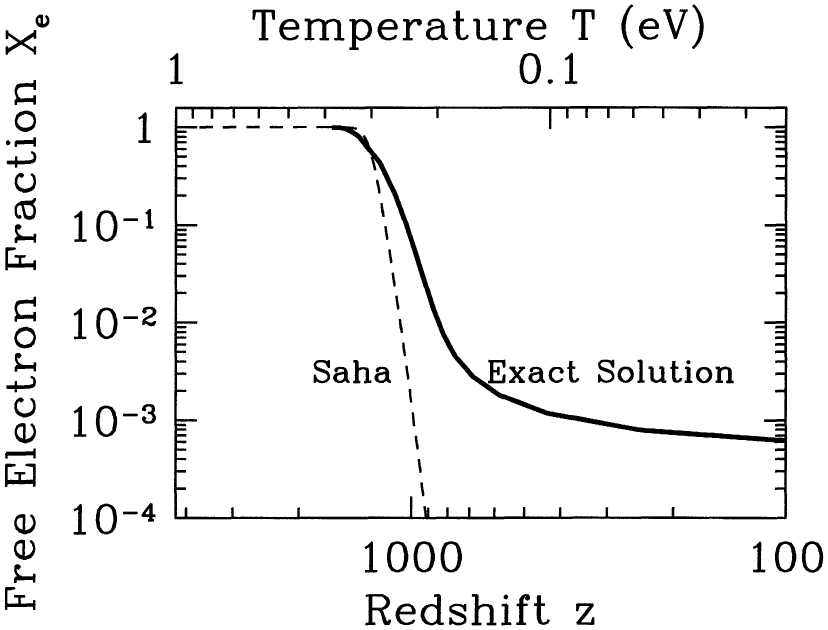
\includegraphics[width=\textwidth]{img/ch-02/ionization.png}
	\caption{The ionization $X_e$ as a function of redshift. Before recombination (at high redshift), the universe is fully ionized with $X_e=1$. The Saha solution assumes thermal equilibrium, which is only valid until recombination. After the freeze-out, a residual ionization fraction ($X_e \approx \num{e-3}$)remains.}
	\label{fig:ionization}
\end{marginfigure}

\subsection{Recombination}

The time of recombination is defined as the time when there are ten times more baryons than electrons: $x_e(z_\text{rec}) = 0.1$. This happens at a temperature of $T_\text{rec} \approx \SI{0.3}{\eV}$ and a redshift of $z \approx 1300$. Note that $T_\text{rec}$ is smaller than the binding energy of hydrogen. This is because recombination is delayed by the high abundance of photons.

\subsection{Decoupling}

The interaction of electrons and photons (in the relevant energy regime) is described by Thomson scattering, with a scattering cross-section of $\sigma_T = \SI{6.65e-25}{\cm\squared}$. The reaction rate is then (see \cref{sec:thermal-history})
\begin{align*}
	\Gamma_T = n_e \sigma_T c,
\end{align*}
where $n_e$ is the number density of electrons, and $c$ the speed of photons. We know that strong coupling occurs as long as $\Gamma_T \gg H$, so we define the moment of decoupling such that
\begin{align*}
	\Gamma_T(z_\text{dec}) = H(z_\text{dec})
\end{align*}
This happens at $z \approx 1100$, $E \approx \SI{0.26}{\eV}$, and $T \approx \SI{3000}{\kelvin}$, after the universe is \SI{380000}{\year} old. Note that $z_\text{dec} < z_\text{rec}$, so decoupling occurs soon after recombination.

After decoupling, the universe is transparent to photons. When an observer today stares into empty space, the photons he measures come from the surface of last scattering, where the photons interacted for the last time during decoupling. This is the cosmic microwave background (CMB), which has a temperature of
\begin{align*}
	T_\text{CMB} = T_\text{dec}\frac{a_0}{a_\text{dec}}
	\approx \SI{3}{\kelvin}
\end{align*}
Measurements of the CMB show a blackbody spectrum with remarkably deviations of $\Delta T / T \approx \num{e-5}$, as can be seen in \cref{fig:cmb}.

\begin{marginfigure}
	\centering
	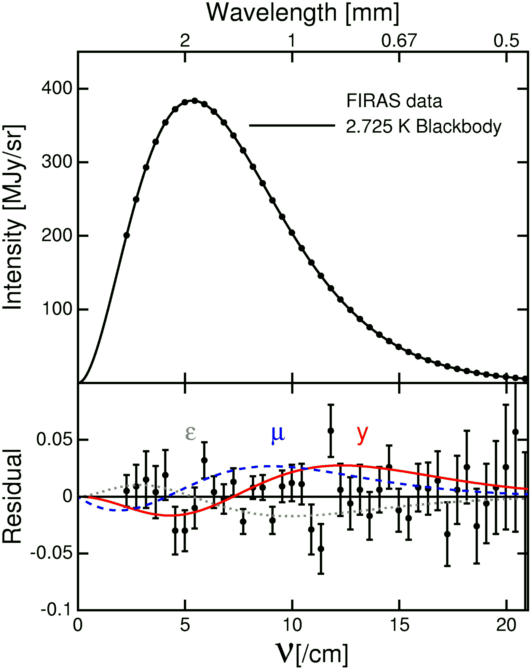
\includegraphics[width=\textwidth]{img/ch-02/cmb.png}
	\caption{The measured spectrum of the cosmic microwave background and a fit with a blackbody spectrum. The residuals show an average deviation of only $\Delta T / T \approx \num{e-5}$.}
	\label{fig:cmb}
\end{marginfigure}




\section{ΛCDM model}


The ΛCDM model is a refinement of the Big Bang model, and it is the standard model of cosmology. Three observational pillars justify this model:
\begin{itemize}
	\item the expansion of the universe,
	\item the big bang nucleosynthesis, and
	\item the cosmic microwave background.
\end{itemize}

According to ΛCDM, the energy content of the universe today is made up of radiation, matter, dark matter, and dark energy. Their contributions today are:
\begin{itemize}
	\item Photons and neutrinos: $\Omega_{\gamma,0} \approx \Omega_{\nu,0}/0.68 \approx \num{2.5e-5} h^{-2}$
	\item Baryons:  $\Omega_{b,0} \approx 0.05$
	\item Dark Matter: $\Omega_{dm,0} \approx 0.25$
	\item Dark Energy: $\Omega_\Lambda \approx 0.7$
\end{itemize}
We now look at the constituents in more detail.

\subsection*{Radiation}

As radiation, we classify those particles that are still relativistic today. Accordingly, they need to have very low mass.
\begin{itemize}
	\item Most photons are part of the CMB and haven a temperature $T\approx \SI{2.73}{\kelvin}$. They contribute only very little to the energy density: $\Omega_{\gamma,0} = \num{2.5e-5}$.
	\item Massless\sidenote{Because of neutrino oscillations, we strongly suspect that neutrinos actually have mass, but it is very low.} neutrinos contribute about the same as photons: $\Omega_{\nu,0} = 0.68 \Omega_{\gamma,0} \approx \num{1.7e-5}$.
\end{itemize}

\subsection*{Baryons}
Baryons from the Big Bang nucleosynthesis contribute $\Omega_b \approx 0.05$. They mostly occur in two forms:
\begin{itemize}
	\item Even though only ten percent of baryons are found in stars, they are the largest fraction of visible matter.
	\item The rest of the baryons is in the form of various phases, such as cold gas, warm gas, and hot gas, both in the intergalactic and the interstellar medium.
\end{itemize}

\subsection*{Dark Matter}
\newacronym{dm}{DM}{dark matter}
\Ac{dm} contributes $\Omega_\text{dm} \approx 0.25$. We know of its existence through its gravitational effects. There is evidence for dark matter in galaxies, galaxy clusters, large scale structure, and many others.

Dark matter is mostly non-baryonic, because baryons are constrained to $\Omega_b \approx 0.05$ by Big Bang nucleosynthesis. Also, the structure formation constraints below rule out baryons as dark matter candidates.
\begin{itemize}
	\item Dark matter is cold (non-relativistic). It is thus called Cold Dark Matter (CDM)
	\item It interacts very weakly, so we can approximate it as non-collisional.
\end{itemize}

A good candidate for dark matter are particles beyond the standard model, such as WIMPs.

Massive Compact Halo Objects (MACHOs), such as black holes, are not good candidates, since objects with masses from $\num{e-6}$ to $15\, M_\sol$ are ruled out.

\subsection*{Dark Energy}
Dark Energy contributes $\Omega_\text{de} \approx 0.7$. It is needed to get a flat geometry for the universe, and to explain the recent acceleration of the expansion of the universe.

From the first Friedmann equation, we know that a constant energy density results in a scale factor $a \propto e^{Ht}$ that is exponentially growing. Consider an effective fluid with equation of state $p_\text{DE} = w \rho_\text{DE} c^2$. We demand $\ddot{a} > 0$, and the second Friedmann equation then yields $w < -1/3$.

There are a few possible candidates:
\begin{itemize}
	\item The cosmological constant $\Lambda$ corresponds to $w=-1$, independent of time.
	\item A model called \emph{quintessence}, which is a dynamical scalar field, would give rise to another form of energy. Since it is dynamical, you can map it to an effective fluid, with a $w$ that varies in time.
	\item There could be a theory of gravity that can improve upon or replace general relativity.
\end{itemize}
Current constraints demand $w = -1$ with an uncertainty of about \SI{5}{\percent}. The cosmological constant is thus a model that is consistent with observations, and it is part of the ΛCDM model.

\subsection*{Summary}
In total, $\Omega_0 \approx 1$, so the universe has a flat geometry. The exact nature of dark energy and dark matter are some of the most pressing questions in fundamental physics.

There are other ingredients to ΛCDM, such as the model of gravity and the choice of initial conditions. A process called inflation is also added, as we will see later.

The ΛCMD model is very successful to fit current observations, but there are some tensions that are starting to emerge with more detailed measurements from cosmological probes.



\section{Problems with ΛCDM}

The ΛCDM model without inflation has a few intrinsic fundamental problems.

\subsection{The horizon problem}
We have defined the particle horizon
\begin{align*}
	\chi_h(t) = \int_0^t \frac{c \dd{t'}}{a(t')},
\end{align*}
which is the maximal comoving distance that a photon could have travelled from the big bang ($t=0$) until time $t$. Let's look at the size of the horizon at decoupling time, where photons scattered for the last time. This corresponds to a redshift $z_\text{dec} \approx 1100$. The integral evaluates to
\begin{align*}
	\chi_h (t_\text{dec}) \approx 180 h^{-1} \, \si{\mega\parsec}
\end{align*}
The corresponding CMB angular scale is
\begin{align*}
	\theta_h
	&= \frac{\chi_h(t_\text{dec})}{r(\chi_\text{dec})} 
	\approx \SI{1.8}{\deg},
\end{align*}
where $r$ is the comoving angular diameter distance.
This is unexpected, because the CMB is extremely homogeneous across the whole sky, even though the photons from different areas of the sky could not have been in causal contact when they scattered! Something must be wrong here.

\subsection{Flatness problem}
We have observationally determined $\Omega_0 \approx 1$, so we have a flat geometry. Let's look at how $\Omega$ varies with time. For this, we can use the Friemann equation:
\begin{align*}
	H(a)^2 = \frac{8\pi G}{3} \rho(a) - \frac{Kc^2}{a^2}
\end{align*}
We look at the deviation of $\Omega$ from $1$:
\begin{align*}
	\frac{1 - \Omega(a)}{\Omega(a)}
	&= \Omega(a)^{-1} - 1\\
	&= -\frac{3Kc^2}{8\pi G \rho(a)a^2}\\
	&\propto
	\begin{cases}
		a^2 &\text{in the radiation era } \rho \propto a^{-4}\\
		a & \text{in the matter era } \rho \propto a^{-3}
	\end{cases}
\end{align*}
Consider time $t_i$ in the radiation era. Then
\begin{align*}
	\frac{\Omega_i^{-1} - 1}{\Omega_0^{-1} - 1}
	&= \frac{\Omega_i^{-1} - 1}{\Omega_\text{eq}^{-1} -1}
	\frac{\Omega_\text{eq}^{-1}-1}{\Omega_0^{-1}-1}\\
	&= 
	\left( \frac{a_i}{a_\text{eq}} \right)^2 
	\left( \frac{a_\text{eq}}{a_0} \right)\\
	&= \left( \frac{T_\text{eq}}{T_i} \right)^2
	\frac{T_0}{T_\text{eq}}
	&& T \propto a^{-1} \text{ for a relativistic gas}
\end{align*}
We choose the Planck time as our starting point:
\begin{align*}
	t_\text{init} &= t_\text{Planck}
	\defeq 
	\left( \frac{\hbar G}{c^5} \right)^{1/2}\\
	T_\text{Planck} &= \SI{e32}{\kelvin}\\
	T_0 &= \SI{3}{\kelvin}\\
	T_\text{eq} &= \SI{e4}{\kelvin} 
\end{align*}
Then
\begin{align*}
	\frac{\Omega_\text{Planck}^{-1} - 1}{\Omega_0^{-1}-1} \approx \num{e-60}
\end{align*}
This means that any deviation of $\Omega$ from $1$ at the Planck time has been amplified by $60$ orders of magnitude until today. This is also called the fine tuning problem, which requires $\Omega=1$ with extreme accuracy at early times. What is the physical explanation of this?


\subsection{Monopole problem}
Consider $T \approx \SI{e14}{\GeV}$, which was the case during the grand unification (GUT) epoch, where the fundamental forces were unified. At these temperatures, there is a phase transition. Before the transition, the forces are unified, and during the transition, there is a spontaneous symmetry breaking. A prediction for topological defects that happen during this transition requires that there should be magnetic monopoles with an enormous density $\Omega_{\text{monopole},0} \approx \num{e11}$. If you still exist, this scenario is obviously ruled out by observations.

\subsection{Structure formation problem}
Today, even though the cosmological principle holds for large distance scales (a few \SI{100}{\mega\parsec}), we still see many structures on various smaller scales in the universe. What were the \enquote{seeds}, the initial perturbations that are responsible for the creation of these structures?

\subsection{Initial condition problem}
All of these problems can be resolved by postulating very special and finely tuned initial conditions. These could arise from physics in the quantum gravity era. The benefit of the inflation model is that all these problems could be resolved without having to resort to quantum gravity.




\section{Inflation}

Inflation is a possible solution for the disparities that we have seen in the previous section. We will tackle them one by one from here.

\subsection{Horizon problem}
We define two things two reformulate the horizon problem:
\begin{itemize}
	\item The size of the forward light cone:
	\begin{align*}
		\chi_f = \int_0 ^{t_\text{ls}} \frac{c \dd{t'}}{a(t')}
	\end{align*}
	\item The size of the past light cone:
	\begin{align*}
		\chi_p = \int_{t_\text{ls}}^{t_0} \frac{c \dd{t'}}{a(t')}
	\end{align*}
	This is the maximum comoving distance that photons could have travelled since last scattering.
\end{itemize}

\begin{figure}
	\centering
	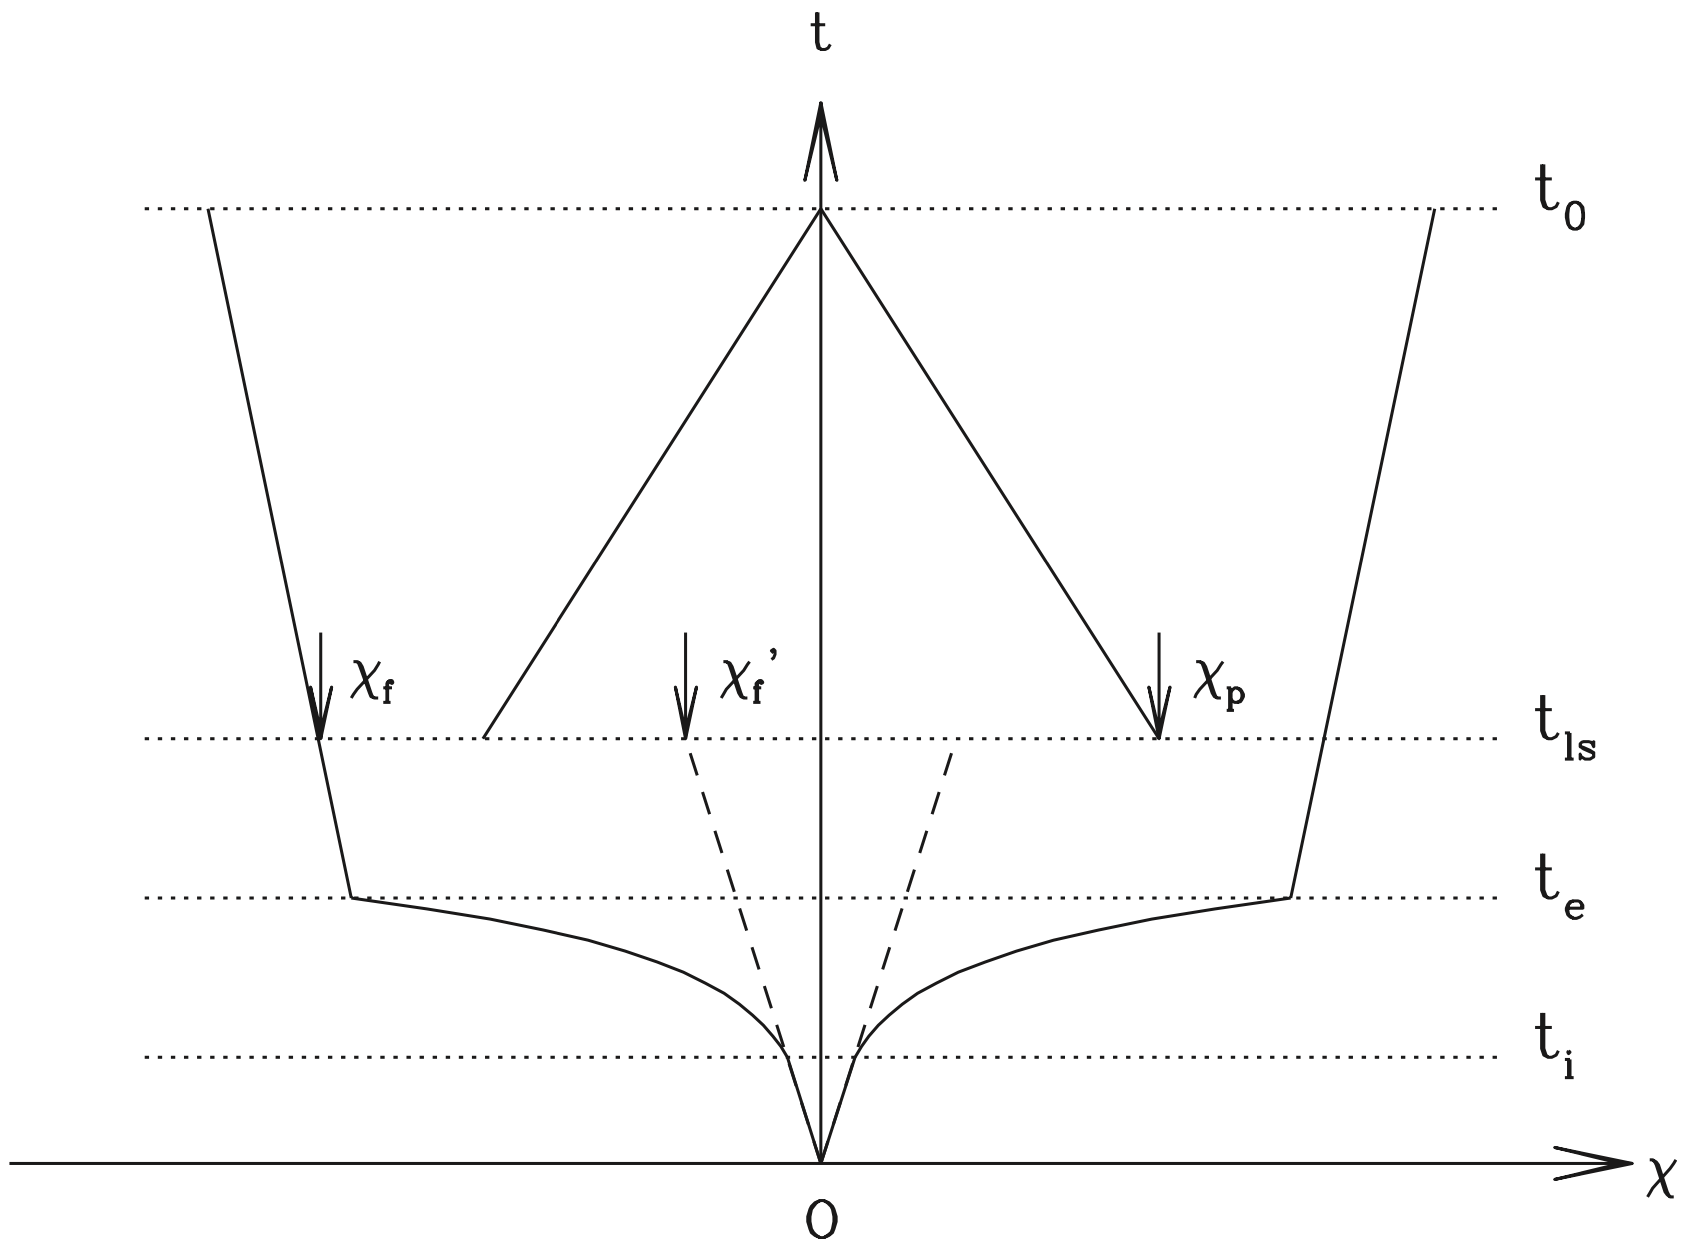
\includegraphics[width=\textwidth]{img/ch-02/inflation.png}
	\caption{The light cone structure in an inflationary universe. Without inflation, the forward light cone (dashed line) would be smaller than our past light cone, $\chi_p$, at the last scattering surface, resulting in causality problems. With a period of inflation from $t_i$ to $t_e$, however, the forward light cone can be larger than the past light cone at $t_\text{ls}$.}
	\label{fig:inflation}
\end{figure}


The horizon problem can be stated mathematically as $\chi_f' < \chi_p$: Regions which are observable today to have similar temperatures were apparently not in causal contact at last scattering. A solution is to increase $\chi_f'$ through a period of accelerated expansion called inflation. A sketch of this is shown in \cref{fig:inflation}.

Let $t_i$ and $t_e$ be the start and end time of inflation, with $\Delta t = t_e - t_i$. We know
\begin{align*}
	\chi_f = \chi_h(t_\text{ls})
	= \int_0^{t_\text{ls}} \frac{c \dd{t'}}{a(t')}
\end{align*}
For vacuum energy, we know that $\rho_\text{vac}(a)$ is constant. We assume that, at early times, there was some kind of vacuum energy which gives us
\begin{align*}
	a \propto e^{Ht} \text{ with } 
	H = \sqrt{8 \pi G \rho_\text{vac}/3} = \text{constant},
\end{align*}
exactly like our derivations for the cosmological constant.
The contribution to $\chi_f$ during inflation is then
\begin{align*}
	\chi_f(t_i,t_e)
	&= \int_{t_i}^{t_e} \frac{c \dd{t'}}{a(t')}\\
	&\propto \frac{1}{H a(t_e)} (e^{H \Delta t} - 1)
\end{align*}
We see that $\chi_f$ grows exponentially during inflation. For how long does inflation have to last to solve our problems? We need $\Delta t > 60 H^{-1}$, or $e^{H \Delta t} < \num{e25}$, if we assume $t_e \approx t_\text{GUT}$. We thus require $a_e/a_i > e^{60}$, or in other words, we need $60$ \enquote{$e$-foldings}.


\subsection{Flatness problem}
One can show that
\begin{align*}
	\frac{\Omega^{-1}(t_e)-1}{\Omega^{-1}(t_i)-1}
	= \frac{a(t_i)}{a(t_e)}
	< \num{e-52}
\end{align*}
assuming $60$ $e$-foldings. As a result, any curvature that was originally there gets flattened by inflation.

\subsection{Monopole problem}
The monopoles are diluted by the expansion during inflation by a factor
\begin{align*}
	\left( \frac{a_e}{a_i} \right)^3 \approx \num{e78},
\end{align*}
so the monopole density after inflation is practically zero.

\subsection{Structure formation problem}
As we will see later, inflation provides a mechanism to generate primordial fluctuations. Microscopic quantum fluctuations are turned into macroscopic classical fluctuations by the rapid expansion.

\subsection{Initial condition problem}
Inflation avoids having to set finely tuned initial conditions, since they will be diluted by the expansion. Quantum gravity is not required to solve this problem.


\subsection{Realization}
Inflation requires vacuum energy, which is realized as a scalar field $\phi(\vec{x}, t)$, called the \emph{inflaton}. The potential of the scalar field is sketched in \cref{fig:false-vacuum}.

\begin{marginfigure}
	\centering
	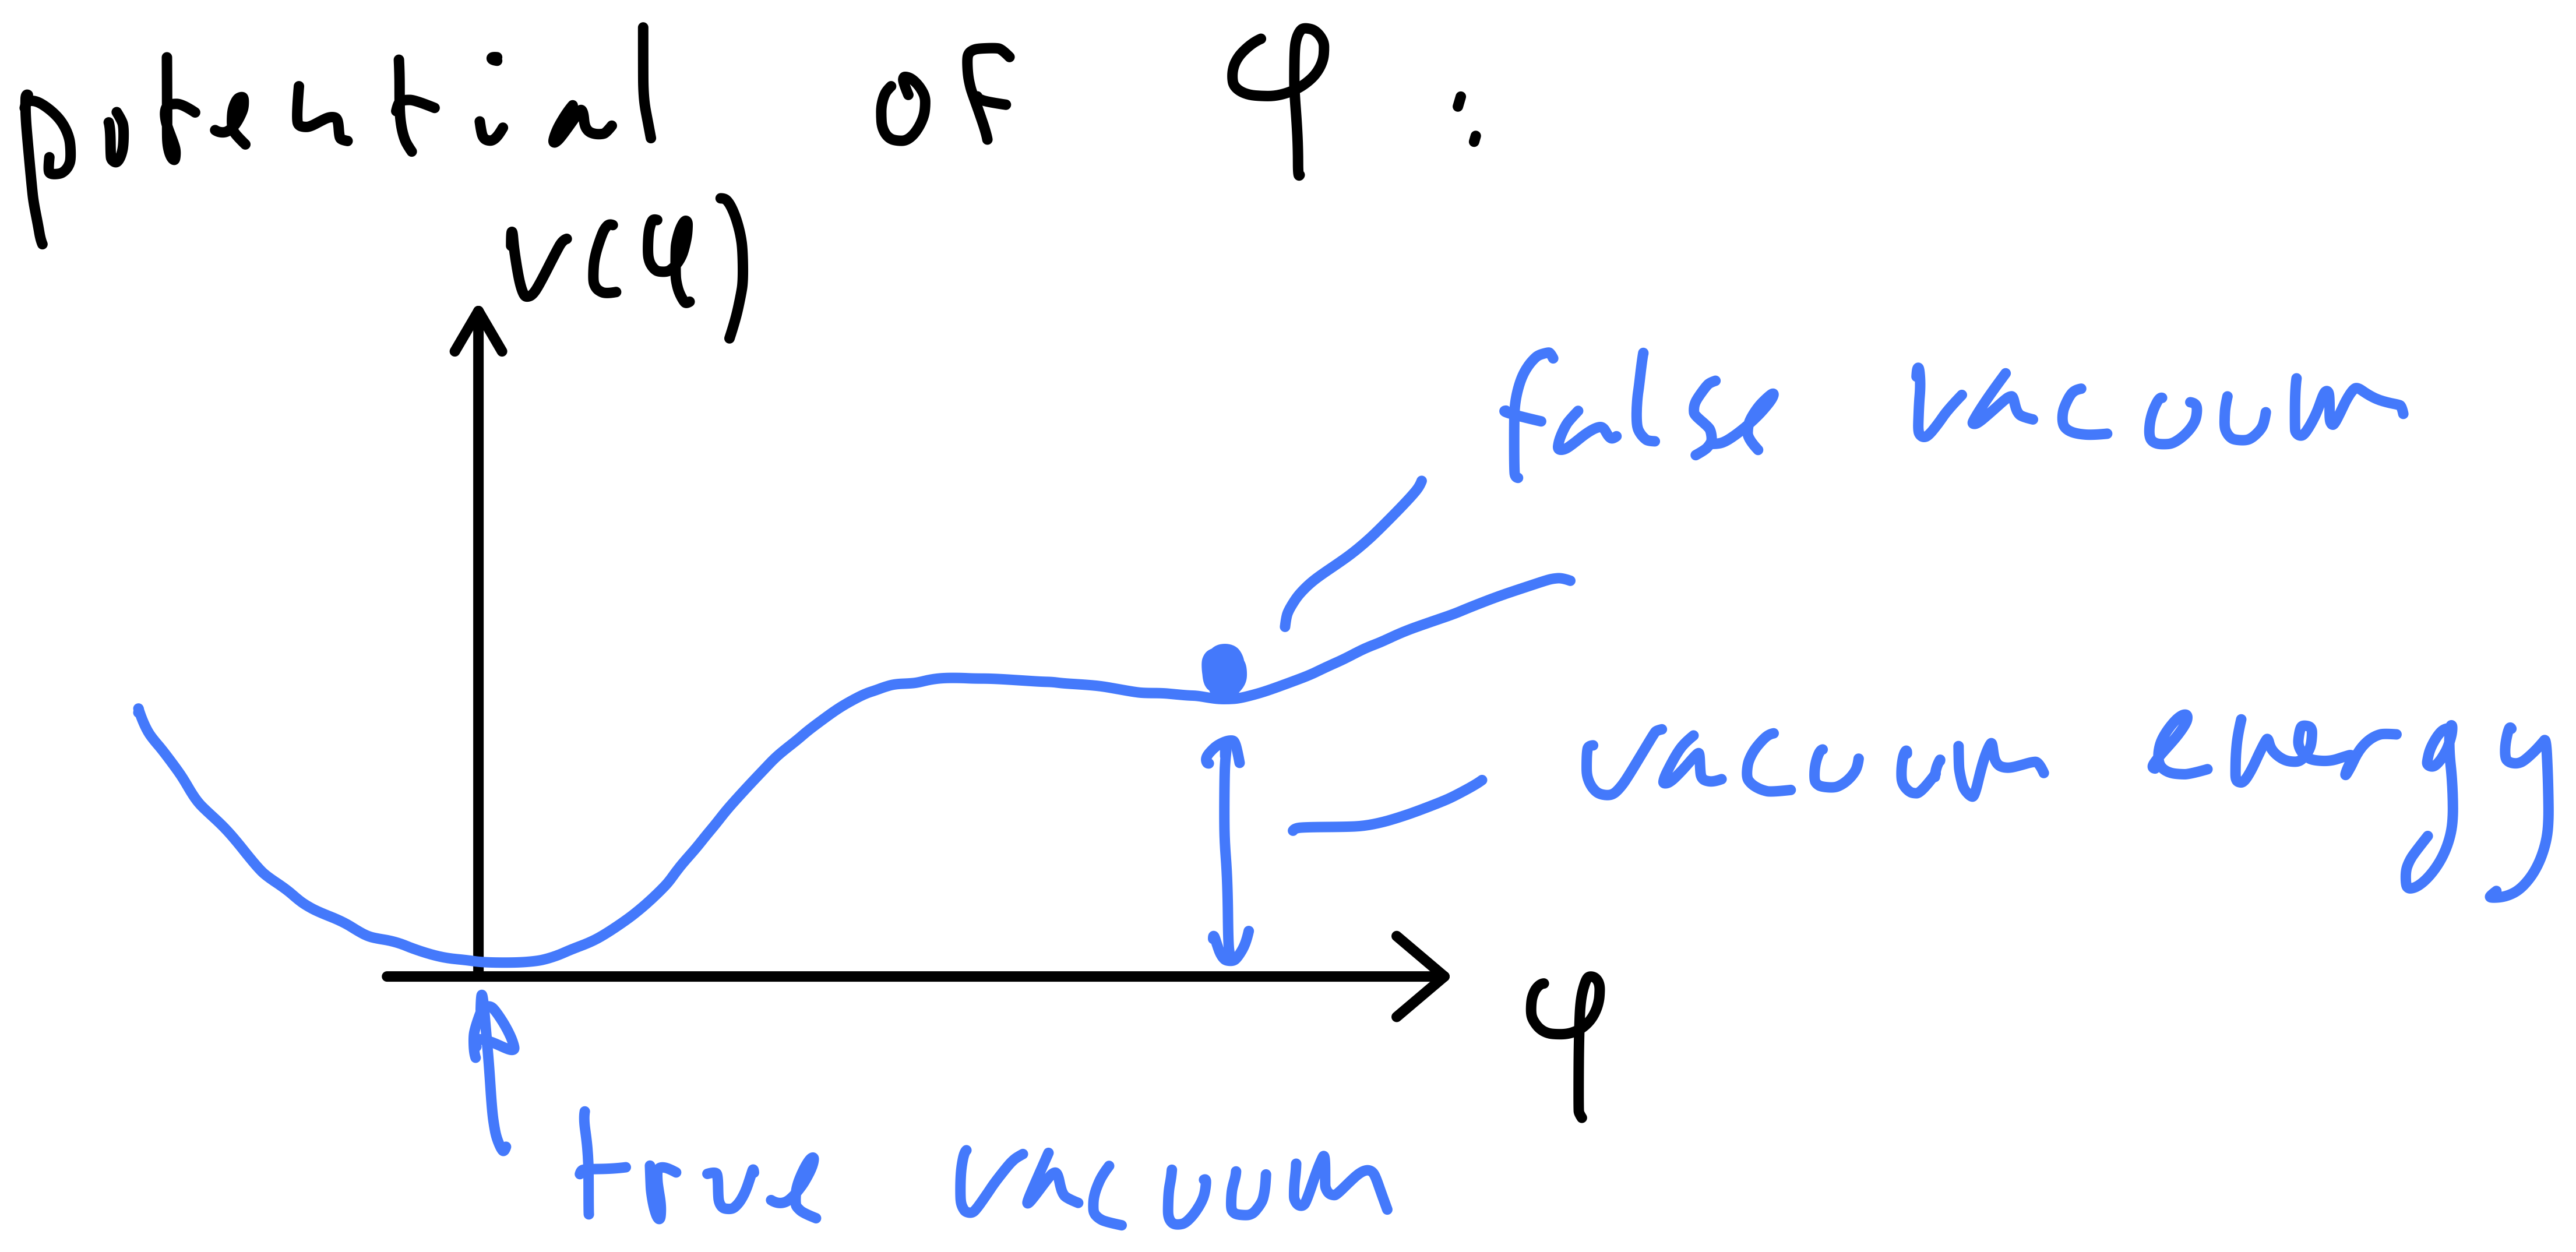
\includegraphics[width=\textwidth]{img/ch-02/false-vacuum.png}
	\caption{The potential of the inflaton field. During inflation, the field moves from its initial false vacuum state to a true vacuum state, which generates vaccum energy.}
	\label{fig:false-vacuum}
\end{marginfigure}

During inflation, $\phi$ is in a false vacuum state at a local minimum  or a flat part of the potential. During the end of inflation, $\phi$ reaches the true vacuum state, which has a lower potential energy. This generates vacuum energy, which in turn drives accelerated expansion.

We impose a \emph{slow roll condition}, which impedes the field from changing too quickly:
\begin{align*}
	\dot{\phi}^2 \ll V(\phi)
\end{align*}
There are several models, some of which are old inflation, new inflation, and chaotic inflation. There are many other models proposed, indicating that inflation is still an ongoing field of research.



